% ==================== 4 单晶硅带轴电子衍射模拟 ====================
\section{单晶硅带轴电子衍射模拟}

\subsection{模拟思路}

第 3 章已经得到每个晶面的消光系数和允许/消光判断。本章的任务是把允许的反射排布到二维倒易面上。电子束沿 $[uvw]$ 方向入射时，属于该带轴的晶面满足晶带方程 $hu+kv+lw=0$，这些晶面的倒易点构成过原点的二维倒易面 $(uvw)^*$。在二维倒易面内选取两条不共线的基矢 $\bm{g}_1=(h_1k_1l_1)^*$、$\bm{g}_2=(h_2k_2l_2)^*$，就可以用整数 $m,n$ 把整个倒易面展开，再由式 \eqref{eq:xy} 和式 \eqref{eq:hkl-mn} 得到每个衍射点的二维坐标和晶面指数。最后，用第 3 章的消光系数表筛选允许的反射，再用二维散点图和三维 Waterfall 图显示。

具体流程如下：
\begin{enumerate}[label=（\arabic*）,leftmargin=2.2em,itemsep=1pt]
  \item 对给定带轴 $[uvw]$，选取两条满足 $hu+kv+lw=0$ 的低指数反射作为 $\bm{g}_1,\bm{g}_2$，并用叉积确认 $\bm{g}_1\times\bm{g}_2\parallel[uvw]$；
  \item 用第 2 章的模板计算 $r_1,r_2,\theta$；
  \item 建立衍射图表格，计算 $x,y,h,k,l$，并把强度初值设为 100，得到几何点阵；
  \item 按第 3 章的消光系数表筛选允许的反射，把消光点删除或置零；
  \item 用二维散点图和三维 Waterfall 图显示结果。
\end{enumerate}

\subsection{基矢的确定与 \texorpdfstring{$r_1$、$r_2$、$\theta$}{r1、r2、theta} 的计算}

带轴确定后，基矢的选法不唯一，但必须满足两个条件：两条反射都满足晶带方程，且叉积 $\bm{g}_1\times\bm{g}_2$ 平行于带轴。需要说明的是，基矢只要求是倒易格点且不共线，并不要求基矢本身是强反射；例如 [111] 的 $(\bar{1}01)^*$ 和 $(0\bar{1}1)^*$ 本身是消光点，但它们的整数组合可以生成 220、422 等允许反射。实际哪些点出现，仍由结构因子决定。以 [421] 带轴为例，$(-120)$ 和 $(-104)$ 都满足
\begin{equation}
4h+2k+l=0,
\end{equation}
因为它们分别给出 $4(-1)+2(2)+0=0$ 和 $4(-1)+2(0)+4=0$；二者的叉积为 $(8,4,2)\parallel[421]$。把这两组指数输入第 2 章的模板，即可得到对应的 $r_1$、$r_2$ 和 $\theta$。图 \ref{fig:basis-calc}(a) 给出了在计算器中输入 $(-120)$、$(-104)$ 的界面，图 \ref{fig:basis-calc}(b) 给出了 $r_1,r_2,\theta$ 的结果，图 \ref{fig:basis-calc}(c) 则是把 $r_1,r_2,\theta$ 代入式 \eqref{eq:xy} 后得到的二维点阵示意。这个 [421] 例子只用于说明方法；本作业要求的五个带轴的基矢和计算结果列于表 \ref{tab:zone-params}。

\begin{figure}[H]
  \centering
  \begin{subfigure}[t]{0.62\linewidth}
    \centering
    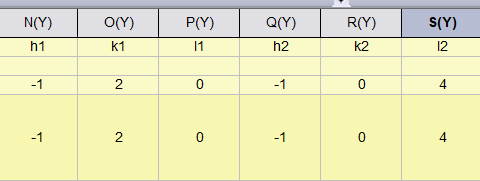
\includegraphics[width=\linewidth]{proc/p06.png}
    \caption{输入 $(-120)$、$(-104)$ 两组晶面}
    \label{fig:basis-calc-a}
  \end{subfigure}\hfill
  \begin{subfigure}[t]{0.14\linewidth}
    \centering
    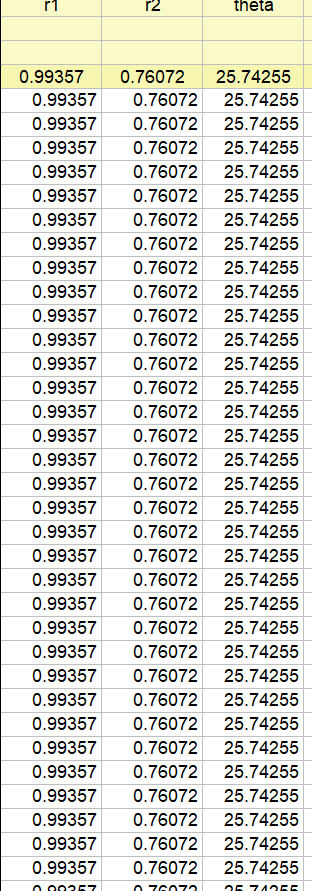
\includegraphics[height=4.6cm]{proc/p07.png}
    \caption{$r_1,r_2,\theta$ 结果}
    \label{fig:basis-calc-b}
  \end{subfigure}

  \vspace{0.3em}
  \begin{subfigure}[t]{0.72\linewidth}
    \centering
    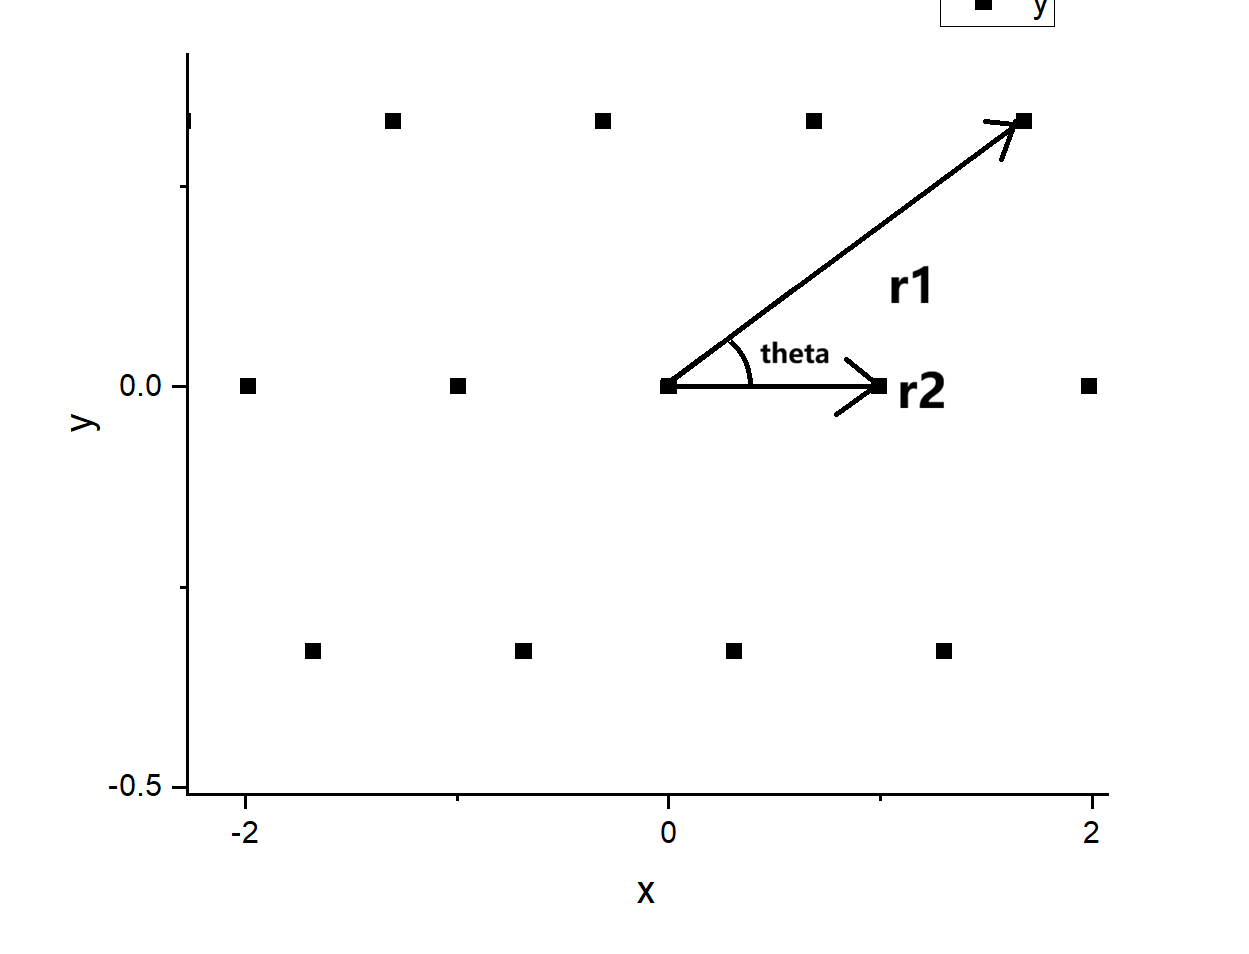
\includegraphics[width=\linewidth]{proc/p08.png}
    \caption{放大后的二维点阵与基矢}
    \label{fig:basis-calc-c}
  \end{subfigure}
  \caption{以 [421] 带轴为例确定基矢：(a) 在计算器中输入 $(-120)$、$(-104)$；(b) 得到 $r_1,r_2,\theta$；(c) 由式 \eqref{eq:xy} 得到的二维点阵。图 (b) 的数值为软件当前表格的显示值，仅用于说明 T--V 三列的位置；五个带轴的实际结果以表 \ref{tab:zone-params} 为准。}
  \label{fig:basis-calc}
\end{figure}

\begin{table}[H]
  \centering
  \caption{五个带轴的基矢、倒易矢量长度、夹角与二维点阵类型（单晶硅，$a=5.43$~\AA）}
  \label{tab:zone-params}
  \small
  \setlength{\tabcolsep}{4pt}
  \renewcommand{\arraystretch}{1.08}
  \begin{tabular}{ccccccc}
    \toprule
    带轴 $[uvw]$ & $\bm{g}_1=(h_1k_1l_1)^*$ & $\bm{g}_2=(h_2k_2l_2)^*$ & $r_1$/\AA$^{-1}$ & $r_2$/\AA$^{-1}$ & $\theta$/$^\circ$ & 二维点阵 \\
    \midrule
    {}[001] & $(100)^*$  & $(010)^*$  & 0.18416 & 0.18416 & 90.0000  & 正方 \\
    {}[111] & $(\bar{1}01)^*$ & $(0\bar{1}1)^*$ & 0.26044 & 0.26044 & 120.0000 & 三角/六方 \\
    {}[332] & $(2\bar{2}0)^*$ & $(04\bar{6})^*$ & 0.52089 & 1.32801 & 113.0935 & 斜方 \\
    {}[334] & $(2\bar{2}0)^*$ & $(08\bar{6})^*$ & 0.52089 & 1.84162 & 124.4499 & 斜方 \\
    {}[345] & $(2\bar{4}2)^*$ & $(\bar{6}22)^*$ & 0.90221 & 1.22159 & 119.4962 & 斜方 \\
    \bottomrule
  \end{tabular}
\end{table}

表 \ref{tab:zone-params} 中的 $r_1,r_2$ 都可由立方晶系的解析式 $r=\sqrt{h^2+k^2+l^2}/a$ 校验。例如 [332] 的 $\bm{g}_2=(04\bar{6})$，$r_2=\sqrt{0^2+4^2+6^2}/5.43=\sqrt{52}/5.43=1.32801$~\AA$^{-1}$；[345] 的 $\bm{g}_1=(2\bar{4}2)$，$r_1=\sqrt{2^2+4^2+2^2}/5.43=\sqrt{24}/5.43=0.90221$~\AA$^{-1}$。夹角也可用式 \eqref{eq:cubic-check} 抽查。若模板结果与解析式不符，应优先检查角度单位和公式中的交叉项。


\subsection{衍射图表格的建立}

新建一个工作表，按 \texttt{r1, r2, theta, m, n, x, y, I, h, k, l} 的顺序建立列，如图 \ref{fig:diff-table}(a)(b) 所示。$m$、$n$ 是二维点阵的整数坐标，图 \ref{fig:diff-table}(c)(d) 中把它们的范围设为 $-5\sim5$，共 $11\times11=121$ 个点。这个范围决定了视场大小：若点阵没有铺满绘图区，可把范围扩大到 $-8\sim8$ 或更大；若只想看中心区域，则可缩小范围。

$x,y$ 两列按式 \eqref{eq:xy} 输入：
\begin{lstlisting}
x = D*A + E*B*COS(C)
y = E*B*SIN(C)
\end{lstlisting}
其中 A、B、C 分别为 $r_1,r_2,\theta$，D、E 分别为 $m,n$。注意 \texttt{COS}、\texttt{SIN} 的自变量是角度，因此角度单位仍须为 Degree。$h,k,l$ 三列按式 \eqref{eq:hkl-mn} 计算。若按附录 A 的推荐列布局，把 $h_1,k_1,l_1$ 放在 L、M、N 列，把 $h_2,k_2,l_2$ 放在 O、P、Q 列，则
\begin{lstlisting}
h = D*L + E*O
k = D*M + E*P
l = D*N + E*Q
\end{lstlisting}
图 \ref{fig:diff-table}(b) 的列名与图 \ref{fig:diff-coords}(c) 的 h、k、l 列就是按这一思路建立的。

\begin{figure}[H]
  \centering
  \begin{subfigure}[t]{0.96\linewidth}
    \centering
    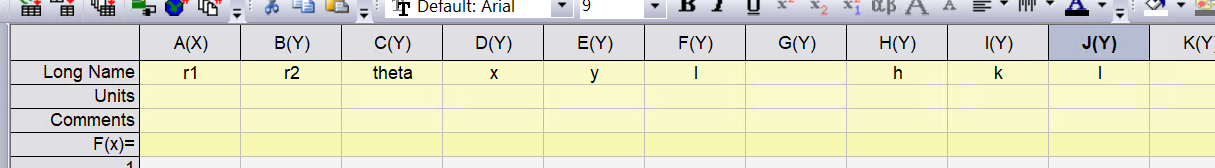
\includegraphics[width=\linewidth]{proc/p09.png}
    \caption{新建衍射图工作表}
    \label{fig:diff-table-a}
  \end{subfigure}

  \vspace{0.25em}
  \begin{subfigure}[t]{0.96\linewidth}
    \centering
    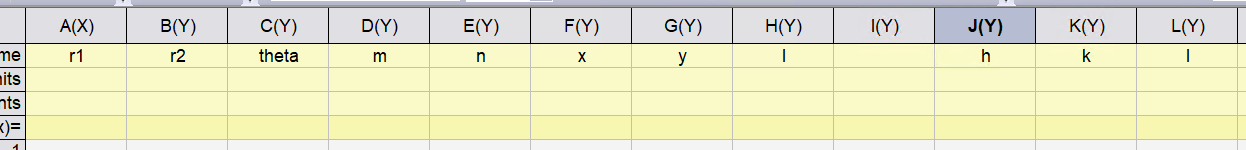
\includegraphics[width=\linewidth]{proc/p10.png}
    \caption{设置列名}
    \label{fig:diff-table-b}
  \end{subfigure}

  \vspace{0.25em}
  \begin{subfigure}[t]{0.32\linewidth}
    \centering
    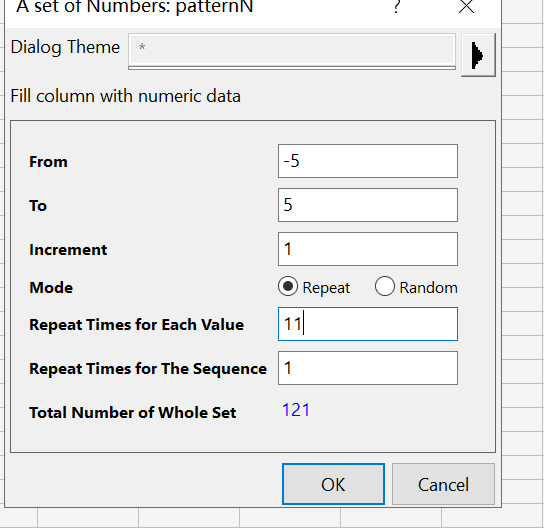
\includegraphics[width=\linewidth]{proc/p11.png}
    \caption{设置 $m$ 的范围}
    \label{fig:diff-table-c}
  \end{subfigure}\hfill
  \begin{subfigure}[t]{0.32\linewidth}
    \centering
    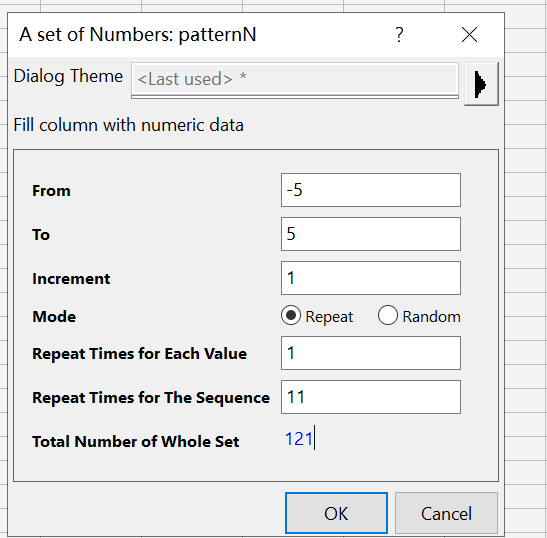
\includegraphics[width=\linewidth]{proc/p12.png}
    \caption{设置 $n$ 的范围}
    \label{fig:diff-table-d}
  \end{subfigure}
  \caption{衍射图表格的建立：(a) 新建工作表；(b) 设置 \texttt{r1, r2, theta, m, n, x, y, I, h, k, l} 等列；(c)(d) 用 \texttt{-5} 到 \texttt{5}、步长 1 填充 $m,n$。}
  \label{fig:diff-table}
\end{figure}

\begin{figure}[H]
  \centering
  \begin{subfigure}[t]{0.20\linewidth}
    \centering
    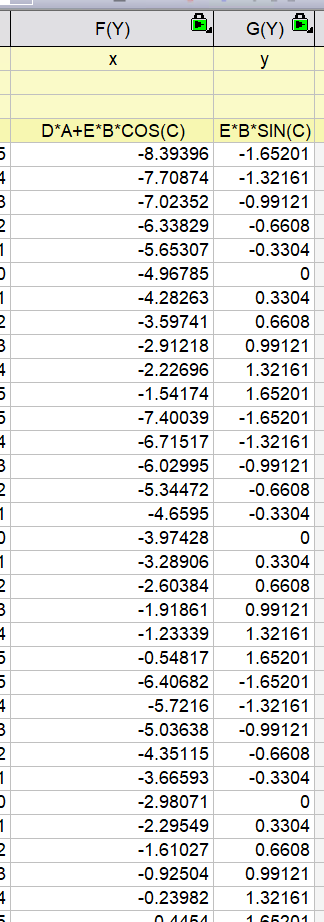
\includegraphics[height=5.2cm]{proc/p13.png}
    \caption{$x,y$ 公式}
    \label{fig:diff-coords-a}
  \end{subfigure}\hfill
  \begin{subfigure}[t]{0.24\linewidth}
    \centering
    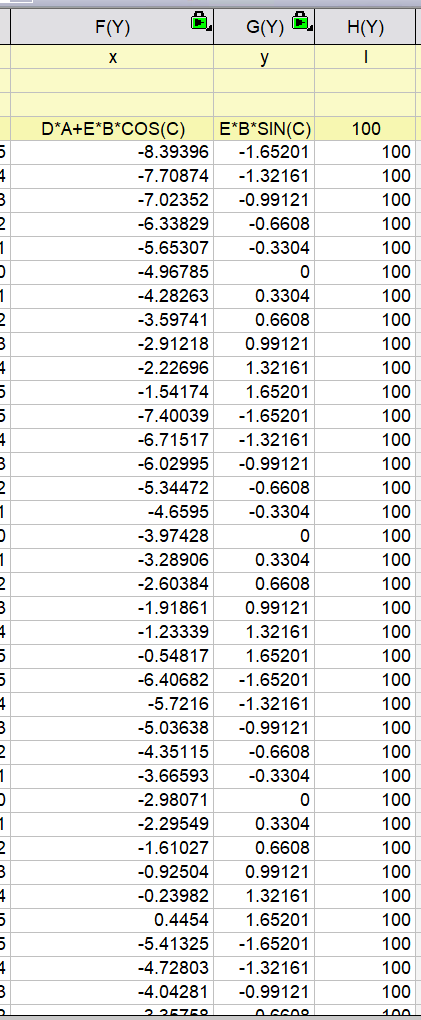
\includegraphics[height=5.2cm]{proc/p14.png}
    \caption{强度初值设为 100}
    \label{fig:diff-coords-b}
  \end{subfigure}\hfill
  \begin{subfigure}[t]{0.20\linewidth}
    \centering
    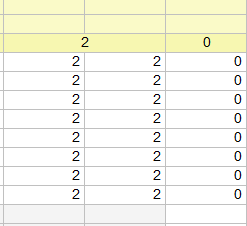
\includegraphics[width=\linewidth]{proc/p15.png}
    \caption{当前 $h,k,l$}
    \label{fig:diff-coords-c}
  \end{subfigure}
  \caption{坐标与指数的计算：(a) 按式 \eqref{eq:xy} 输入 $x,y$；(b) 几何模拟时把 $I$ 统一设为 100；(c) 当前衍射点的 $h,k,l$。}
  \label{fig:diff-coords}
\end{figure}


\subsection{绘图与五个带轴的结果}

\begin{figure}[H]
  \centering
  \begin{subfigure}[t]{0.34\linewidth}
    \centering
    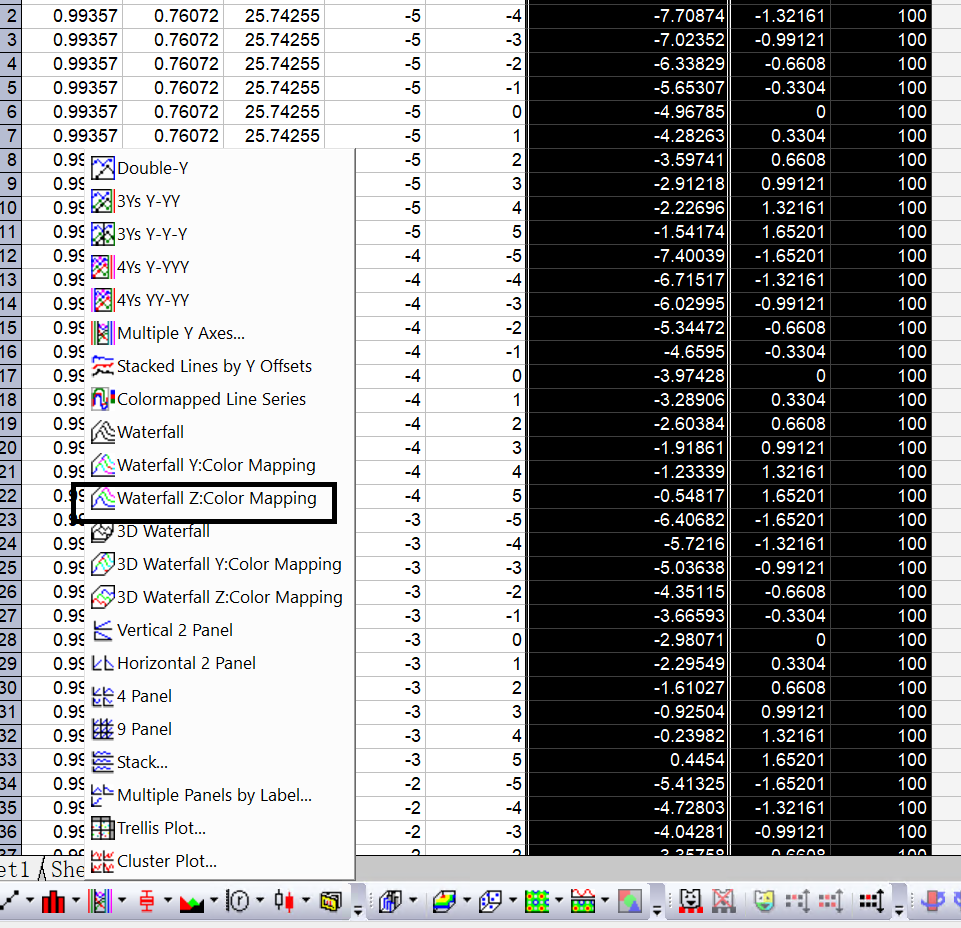
\includegraphics[width=\linewidth]{proc/p22.png}
    \caption{选择 3D Waterfall（WaterfallZ）}
    \label{fig:plot-setup-a}
  \end{subfigure}\hfill
  \begin{subfigure}[t]{0.46\linewidth}
    \centering
    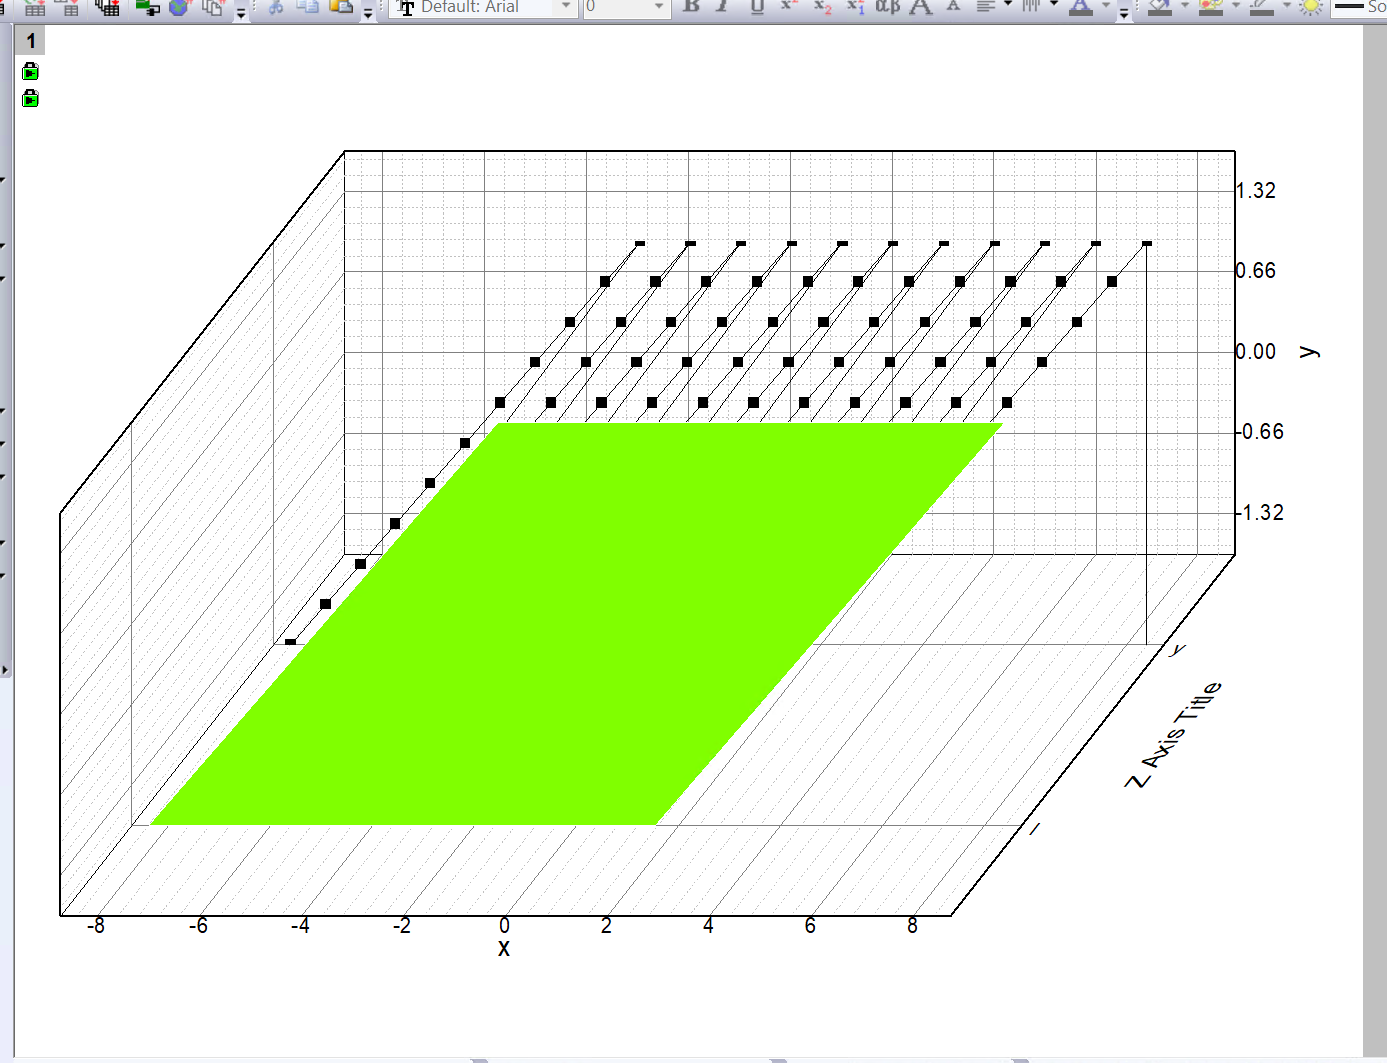
\includegraphics[width=\linewidth]{proc/p23.png}
    \caption{三维 Waterfall 示例}
    \label{fig:plot-setup-b}
  \end{subfigure}

  \vspace{0.3em}
  \begin{subfigure}[t]{0.44\linewidth}
    \centering
    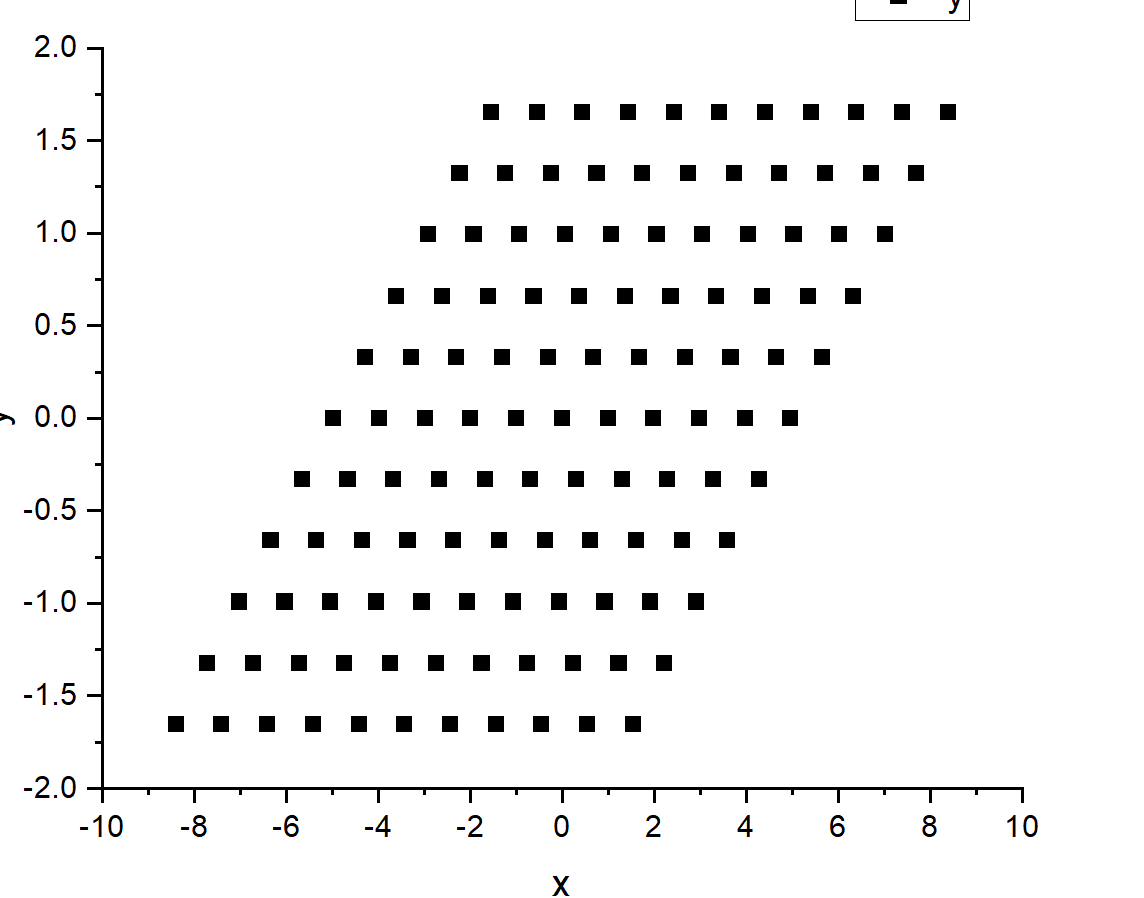
\includegraphics[width=\linewidth]{proc/p24.png}
    \caption{二维散点示例}
    \label{fig:plot-setup-c}
  \end{subfigure}
  \caption{Origin 绘图设置与示例：(a) 选择 3D Waterfall（WaterfallZ）；(b) 三维 Waterfall 图（绿色平面为默认填充对象）；(c) 二维散点图（示例为 [421] 带轴）。}
  \label{fig:plot-setup}
\end{figure}

有了 $x,y,I$ 三列，就可以绘图。二维图选择 \texttt{Plot $\rightarrow$ Scatter}，以 $x$ 为横轴、$y$ 为纵轴；三维图选择 \texttt{Plot $\rightarrow$ 3D Waterfall}，以 $x,y$ 为平面坐标、$I$ 为高度。图 \ref{fig:plot-setup}(a) 是 Waterfall 的设置界面，图 \ref{fig:plot-setup}(b) 是三维示例，图 \ref{fig:plot-setup}(c) 是二维散点示例。三维图中出现的绿色平面是 Origin 默认生成的填充对象（或当前选中的图层），它会遮挡部分数据；正式绘图时应在 \texttt{Plot Details} 中删除该对象，或把填充透明度设为 0。本文保留原始截图，以说明这一常见问题。

以下五组图分别给出 [001]、[111]、[332]、[334]、[345] 五个带轴的计算界面、坐标复制、二维散点图和三维 Waterfall 图。每组图中的 (a) 是 Origin 计算模板中输入的基矢与 $r_1,r_2,\theta$，(b) 是把 $r_1,r_2,\theta$ 复制到衍射图表格后的列数据，(c)(d) 是最终的点阵图。由于几何模拟把 $I$ 统一设为 100，(c)(d) 中所有点的高度相同；实际强度需按第 3 章的消光系数表筛选，消光点应删除或置零。

\subsubsection{[001] 带轴}

[001] 带轴的基矢为 $\bm{g}_1=(100)^*$、$\bm{g}_2=(010)^*$，$r_1=r_2=0.18416$~\AA$^{-1}$，$\theta=90^\circ$。二维点阵是正方形，具有 4 次对称；$m,n$ 取 $-5\sim5$ 时，视场内约有 $11\times11$ 个点。由于金刚石结构的消光，实际允许的反射是 220、400、440、620 等，100、110、200 等不出现。图 \ref{fig:zone001}(c)(d) 中所有点高度相同，是因为几何模拟把 $I$ 统一设为 100；若把 $I$ 换成结构因子列，100、110、200 等点会消失，只剩 220、400 等强点。

\begin{figure}[H]
  \centering
  \begin{subfigure}[t]{0.64\linewidth}
    \centering
    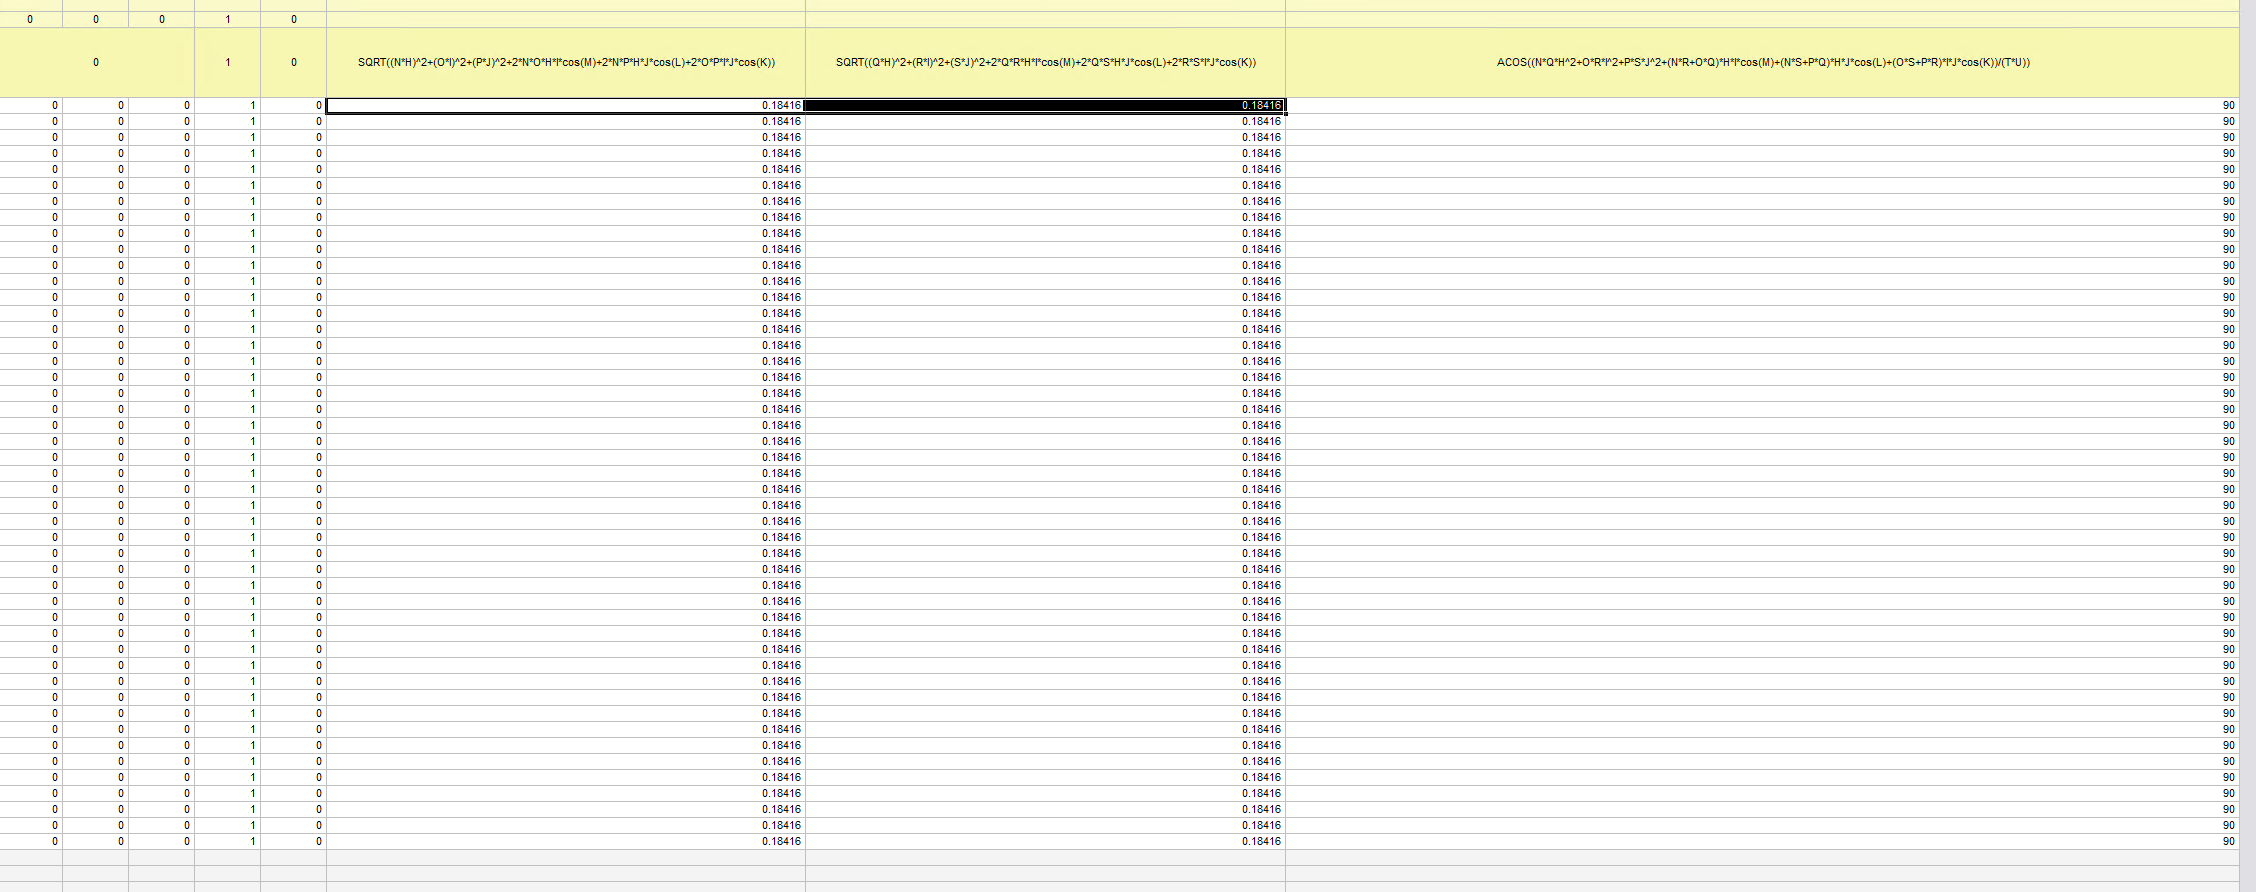
\includegraphics[width=\linewidth]{zone001/zone001_a.png}
    \caption{基矢与 $r_1,r_2,\theta$}
    \label{fig:zone001-a}
  \end{subfigure}\hfill
  \begin{subfigure}[t]{0.14\linewidth}
    \centering
    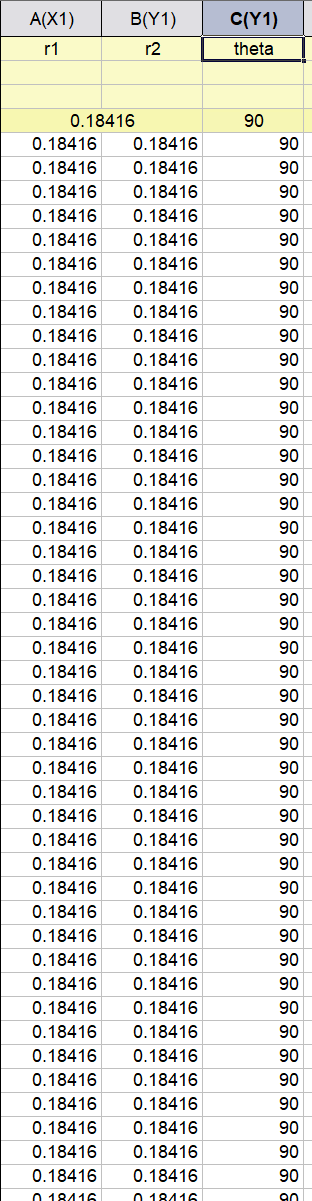
\includegraphics[height=4.3cm]{zone001/zone001_b.png}
    \caption{坐标复制}
    \label{fig:zone001-b}
  \end{subfigure}

  \vspace{0.3em}
  \begin{subfigure}[t]{0.48\linewidth}
    \centering
    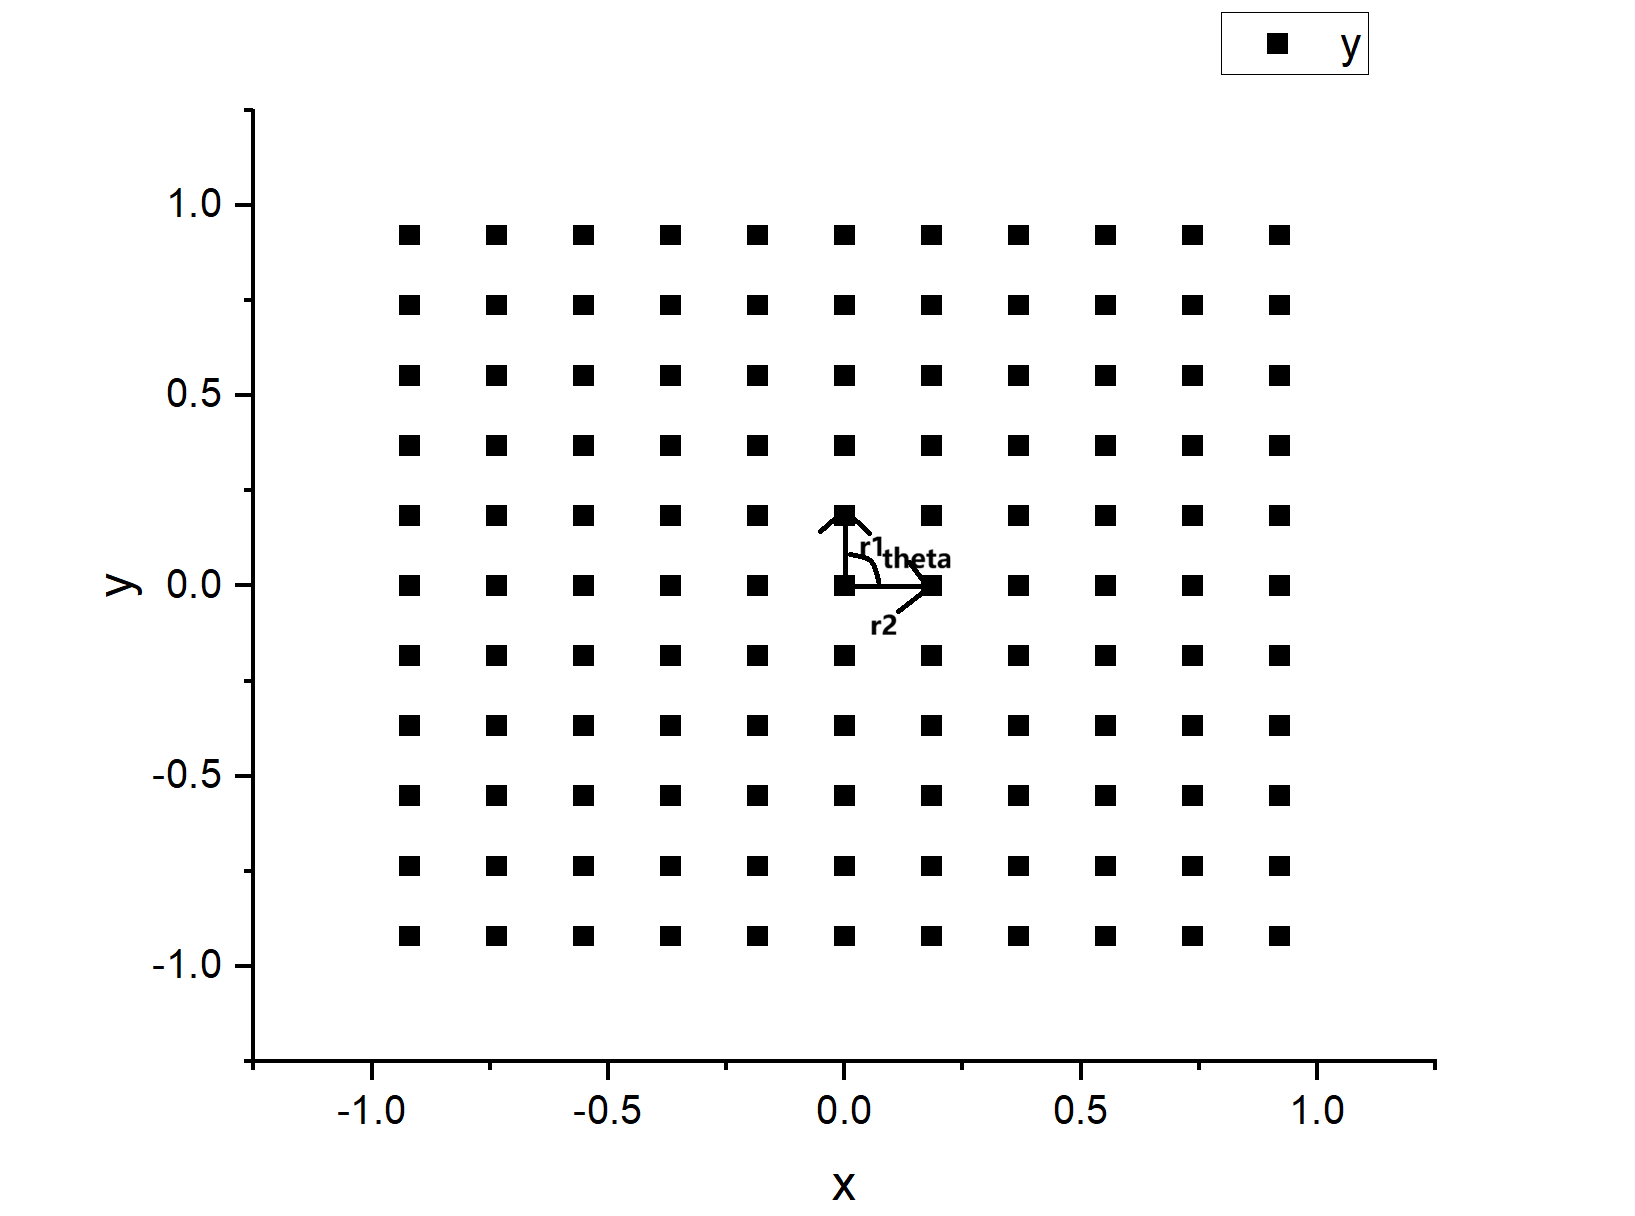
\includegraphics[width=\linewidth]{zone001/zone001_c.png}
    \caption{二维散点图}
    \label{fig:zone001-c}
  \end{subfigure}\hfill
  \begin{subfigure}[t]{0.48\linewidth}
    \centering
    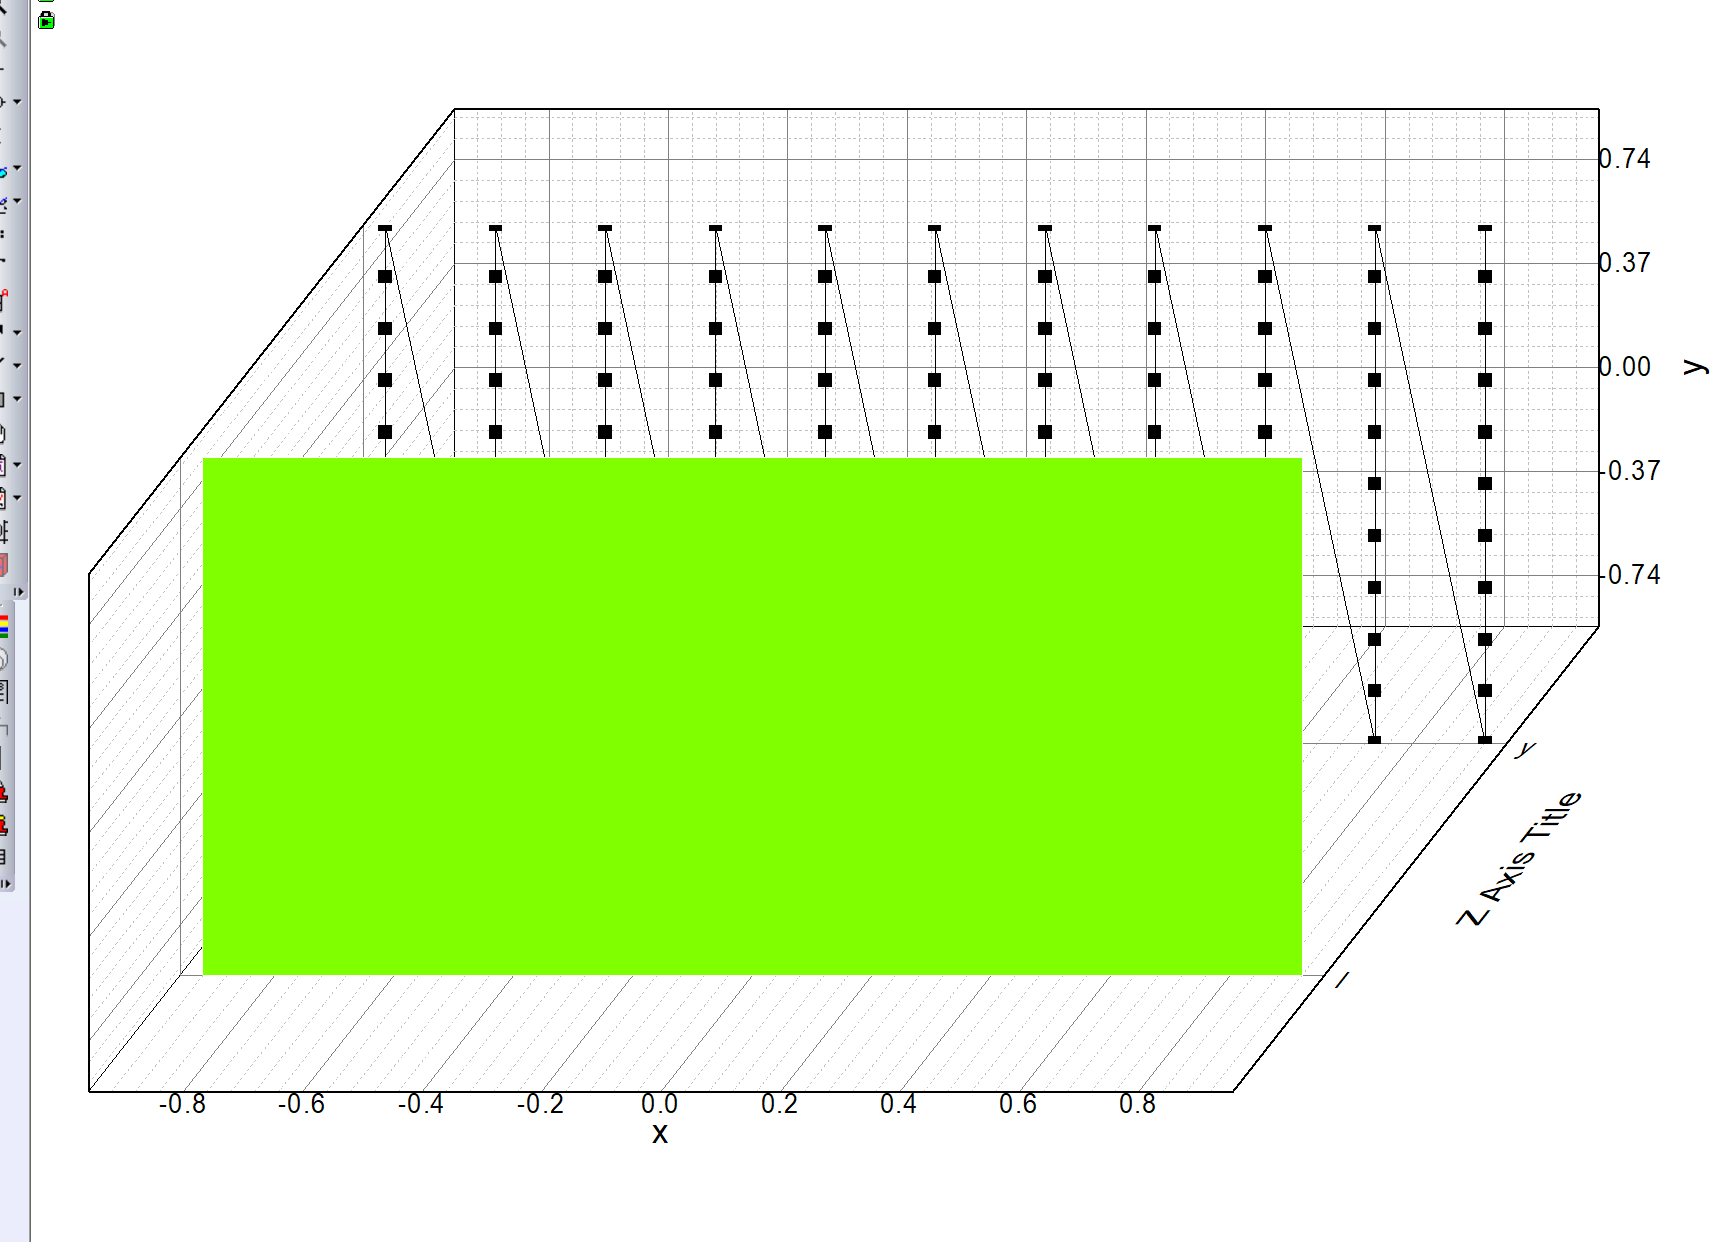
\includegraphics[width=\linewidth]{zone001/zone001_d.png}
    \caption{三维 Waterfall 图}
    \label{fig:zone001-d}
  \end{subfigure}
  \caption{[001] 带轴电子衍射模拟：(a) 基矢 $(100)^*$、$(010)^*$ 与 $r_1=r_2=0.18416$~\AA$^{-1}$、$\theta=90^\circ$；(b) 把 $r_1,r_2,\theta$ 复制到衍射图表格；(c) 正方形二维点阵；(d) 三维 Waterfall 图（绿色平面为默认填充对象）。}
  \label{fig:zone001}
\end{figure}

\subsubsection{[111] 带轴}

[111] 带轴的基矢为 $\bm{g}_1=(\bar{1}01)^*$、$\bm{g}_2=(0\bar{1}1)^*$，$r_1=r_2=0.26044$~\AA$^{-1}$，$\theta=120^\circ$。二维点阵是三角/六方点阵，基矢夹角 $120^\circ$；点阵本身具有 6 次对称，实际衍射强度受结构因子调制，可能出现 3 次对称。允许的反射为 220、422、440 等；111 本身不满足 $hu+kv+lw=0$，属于高阶劳厄带，不在零阶劳厄区内。与 [001] 相比，[111] 的点阵更疏，斑点呈六方排列。

\begin{figure}[H]
  \centering
  \begin{subfigure}[t]{0.64\linewidth}
    \centering
    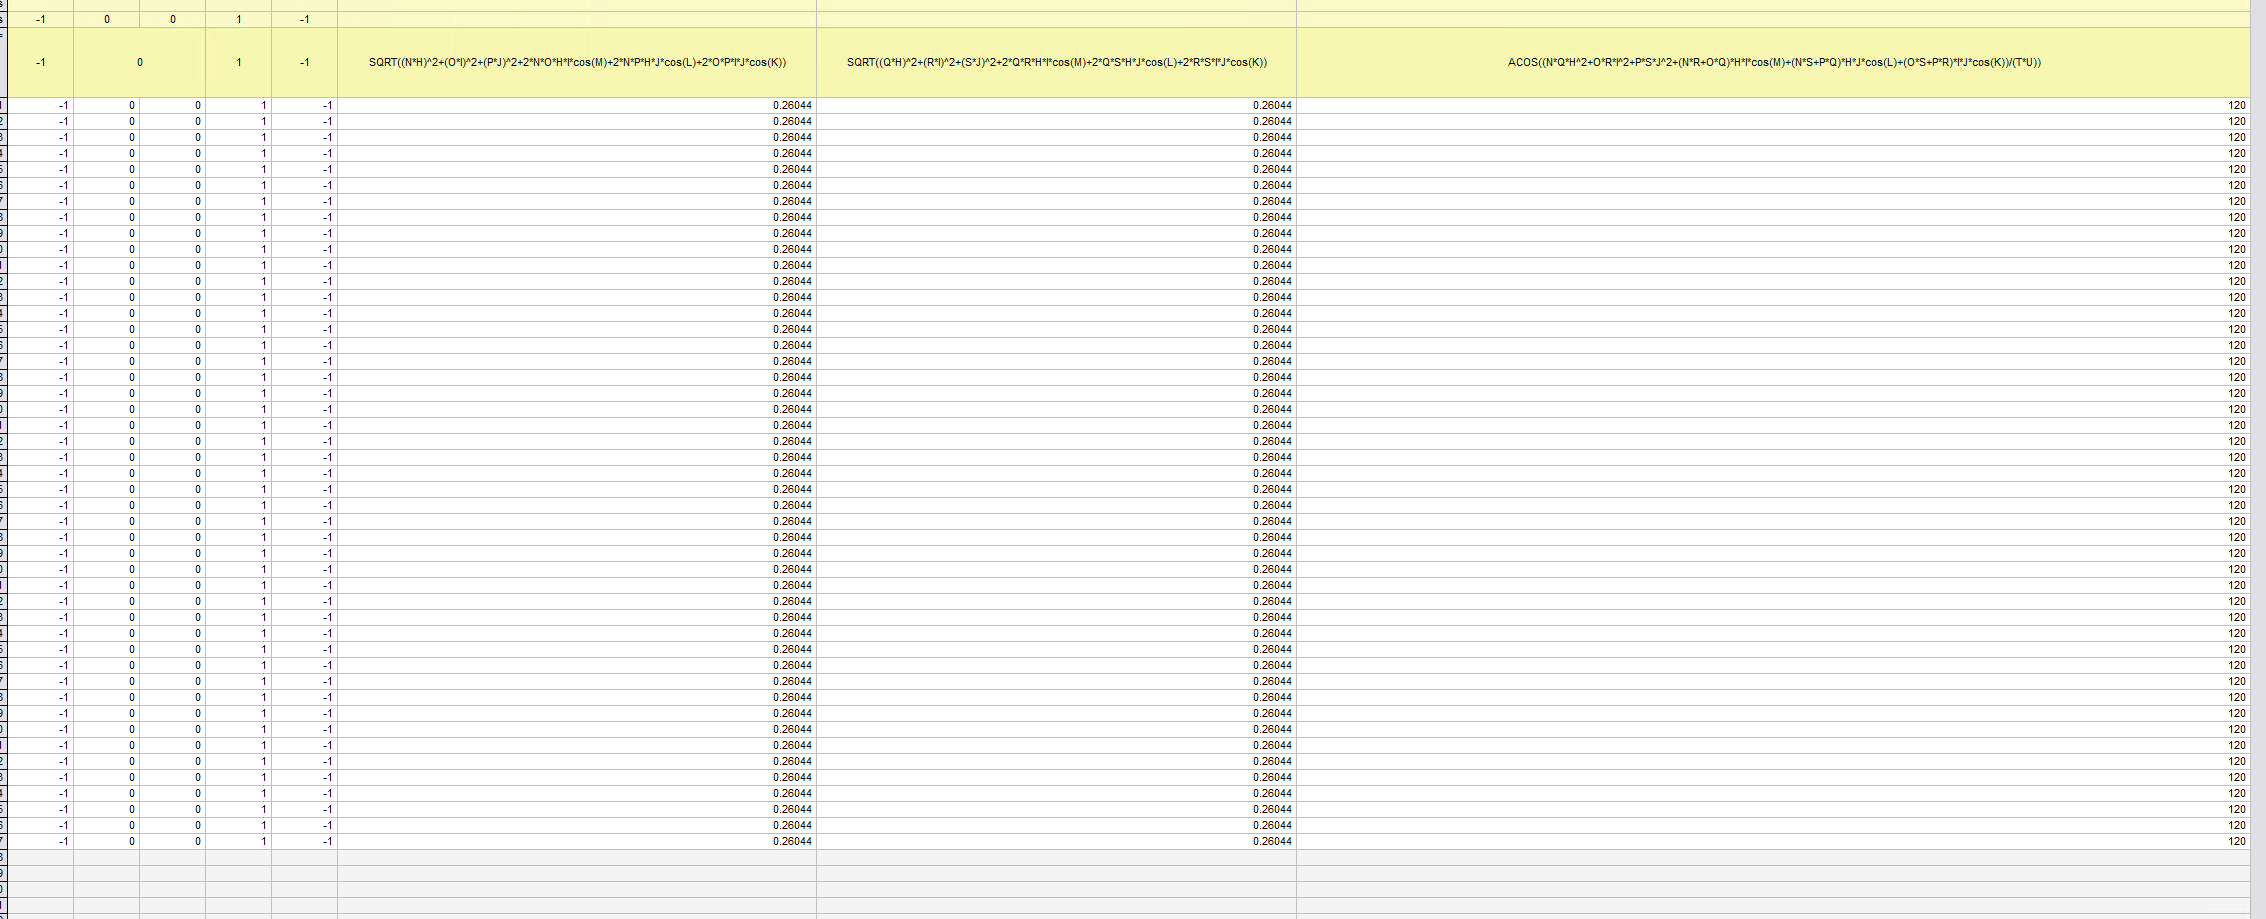
\includegraphics[width=\linewidth]{zone111/zone111_a.png}
    \caption{基矢与 $r_1,r_2,\theta$}
    \label{fig:zone111-a}
  \end{subfigure}\hfill
  \begin{subfigure}[t]{0.14\linewidth}
    \centering
    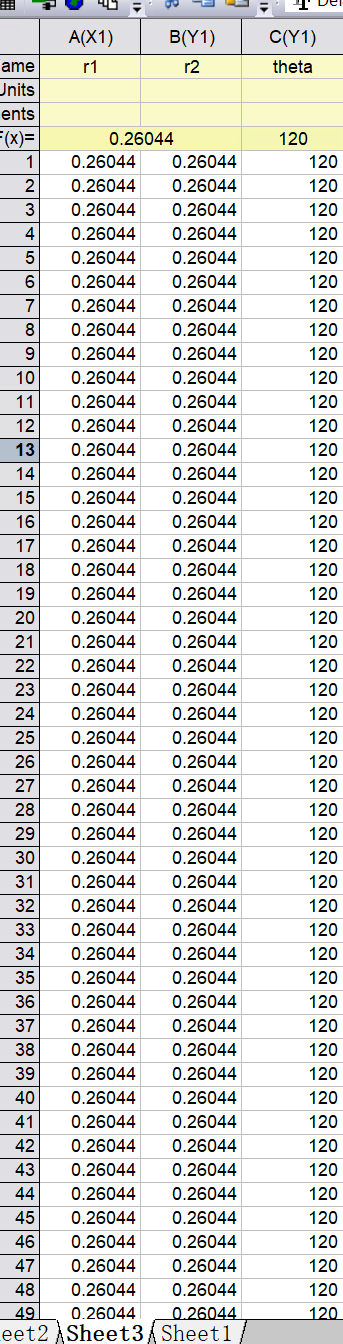
\includegraphics[height=4.3cm]{zone111/zone111_b.png}
    \caption{坐标复制}
    \label{fig:zone111-b}
  \end{subfigure}

  \vspace{0.3em}
  \begin{subfigure}[t]{0.48\linewidth}
    \centering
    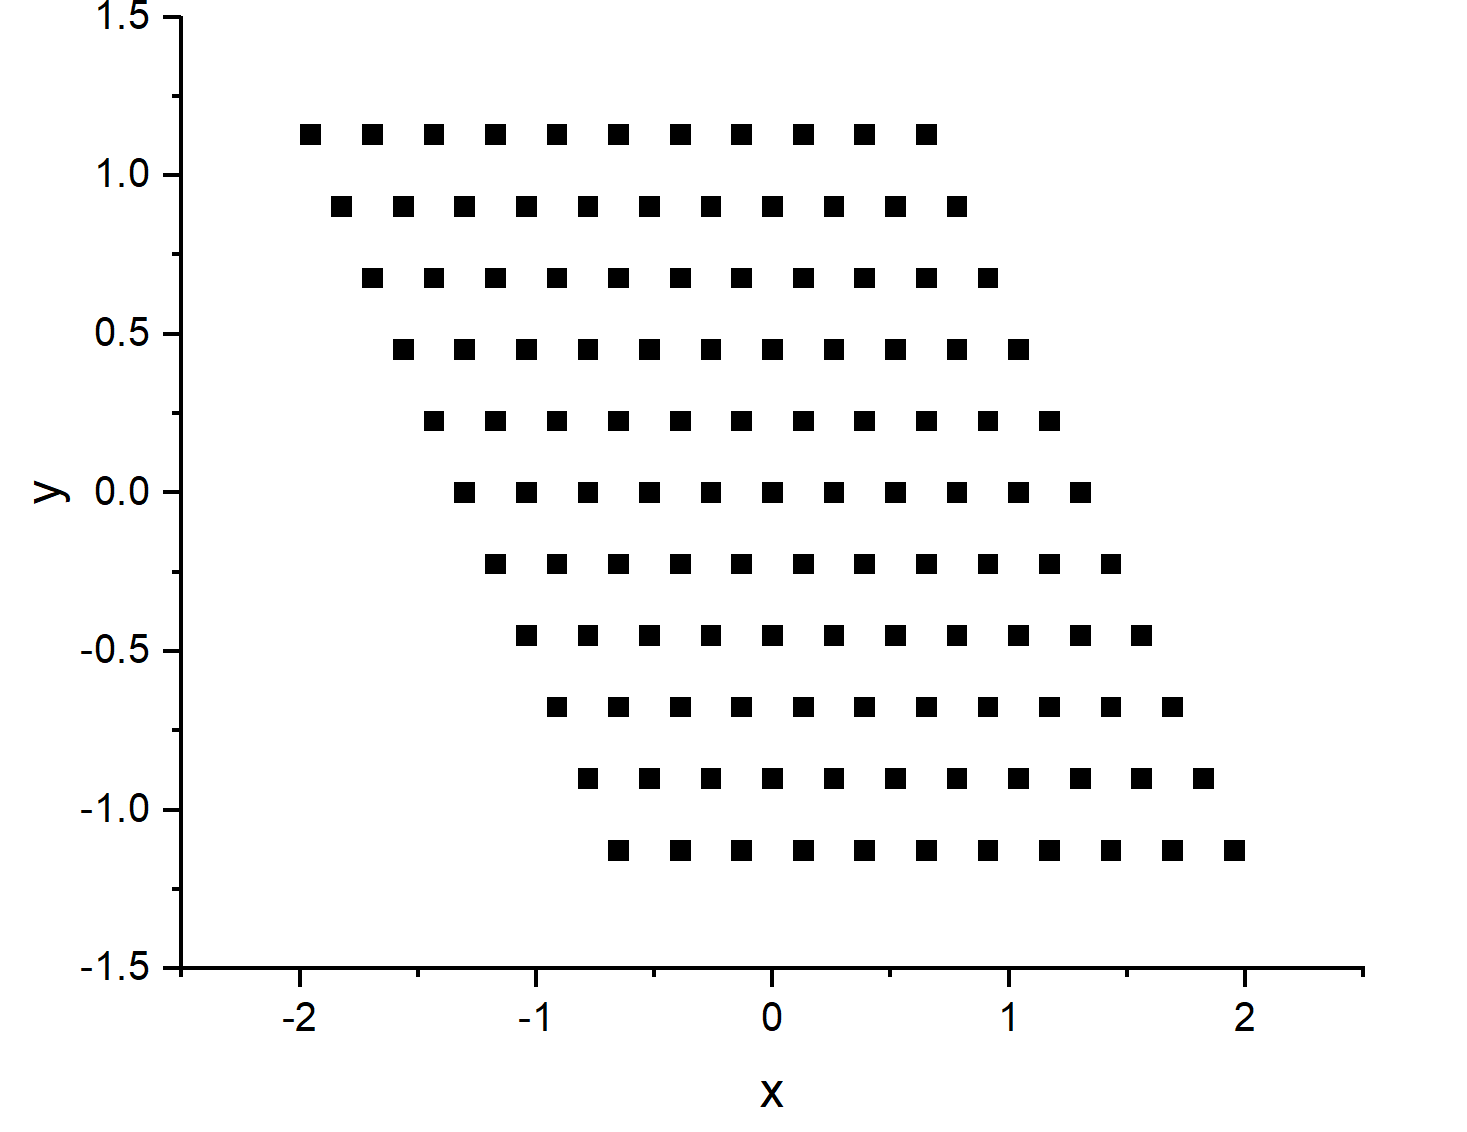
\includegraphics[width=\linewidth]{zone111/zone111_c.png}
    \caption{二维散点图}
    \label{fig:zone111-c}
  \end{subfigure}\hfill
  \begin{subfigure}[t]{0.48\linewidth}
    \centering
    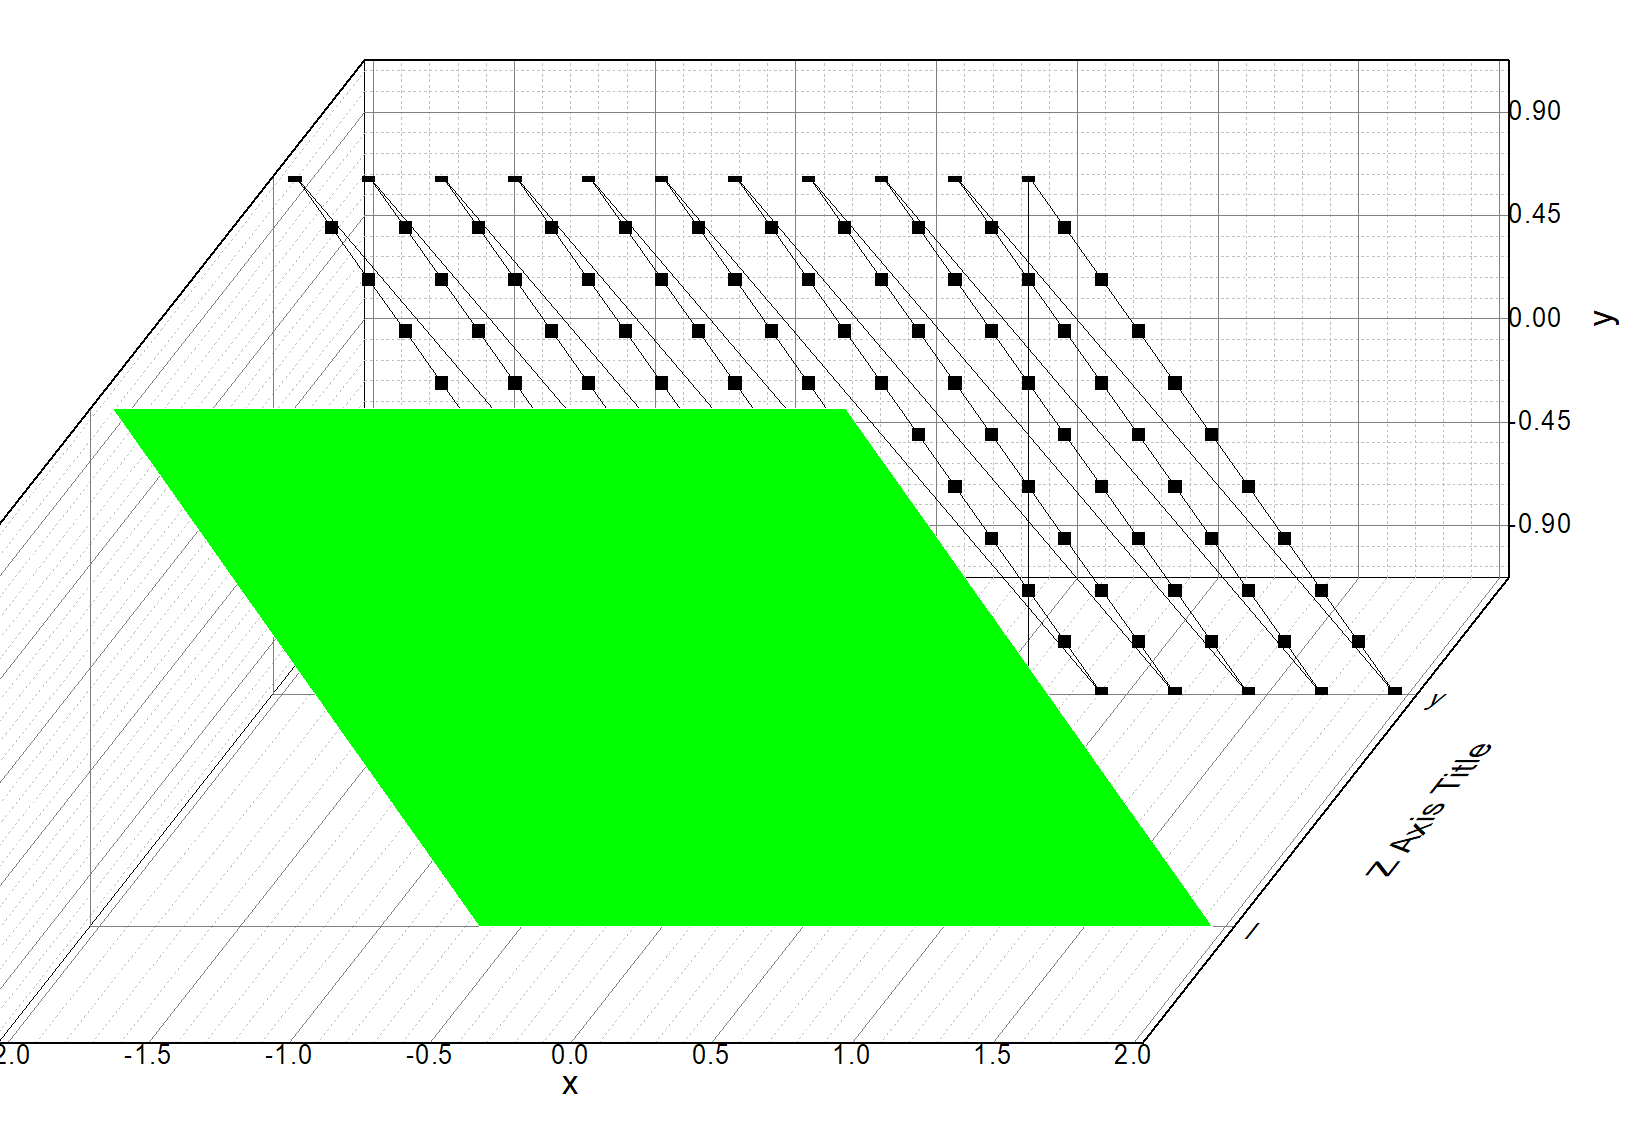
\includegraphics[width=\linewidth]{zone111/zone111_d.png}
    \caption{三维 Waterfall 图}
    \label{fig:zone111-d}
  \end{subfigure}
  \caption{[111] 带轴电子衍射模拟：(a) 基矢 $(\bar{1}01)^*$、$(0\bar{1}1)^*$ 与 $r_1=r_2=0.26044$~\AA$^{-1}$、$\theta=120^\circ$；(b) 坐标复制；(c) 三角/六方二维点阵；(d) 三维 Waterfall 图。}
  \label{fig:zone111}
\end{figure}

\subsubsection{[332] 带轴}

[332] 带轴的基矢为 $\bm{g}_1=(2\bar{2}0)^*$、$\bm{g}_2=(04\bar{6})^*$，$r_1=0.52089$~\AA$^{-1}$，$r_2=1.32801$~\AA$^{-1}$，$\theta=113.0935^\circ$。二维点阵为斜方/平行四边形，夹角大于 $90^\circ$；第二基矢较长，因此沿该方向的点间距较大。允许的反射包括 220、311、331、440 等。与 [001]、[111] 相比，[332] 的对称性明显降低，点阵不再具有 4 次或 6 次对称。

\begin{figure}[H]
  \centering
  \begin{subfigure}[t]{0.64\linewidth}
    \centering
    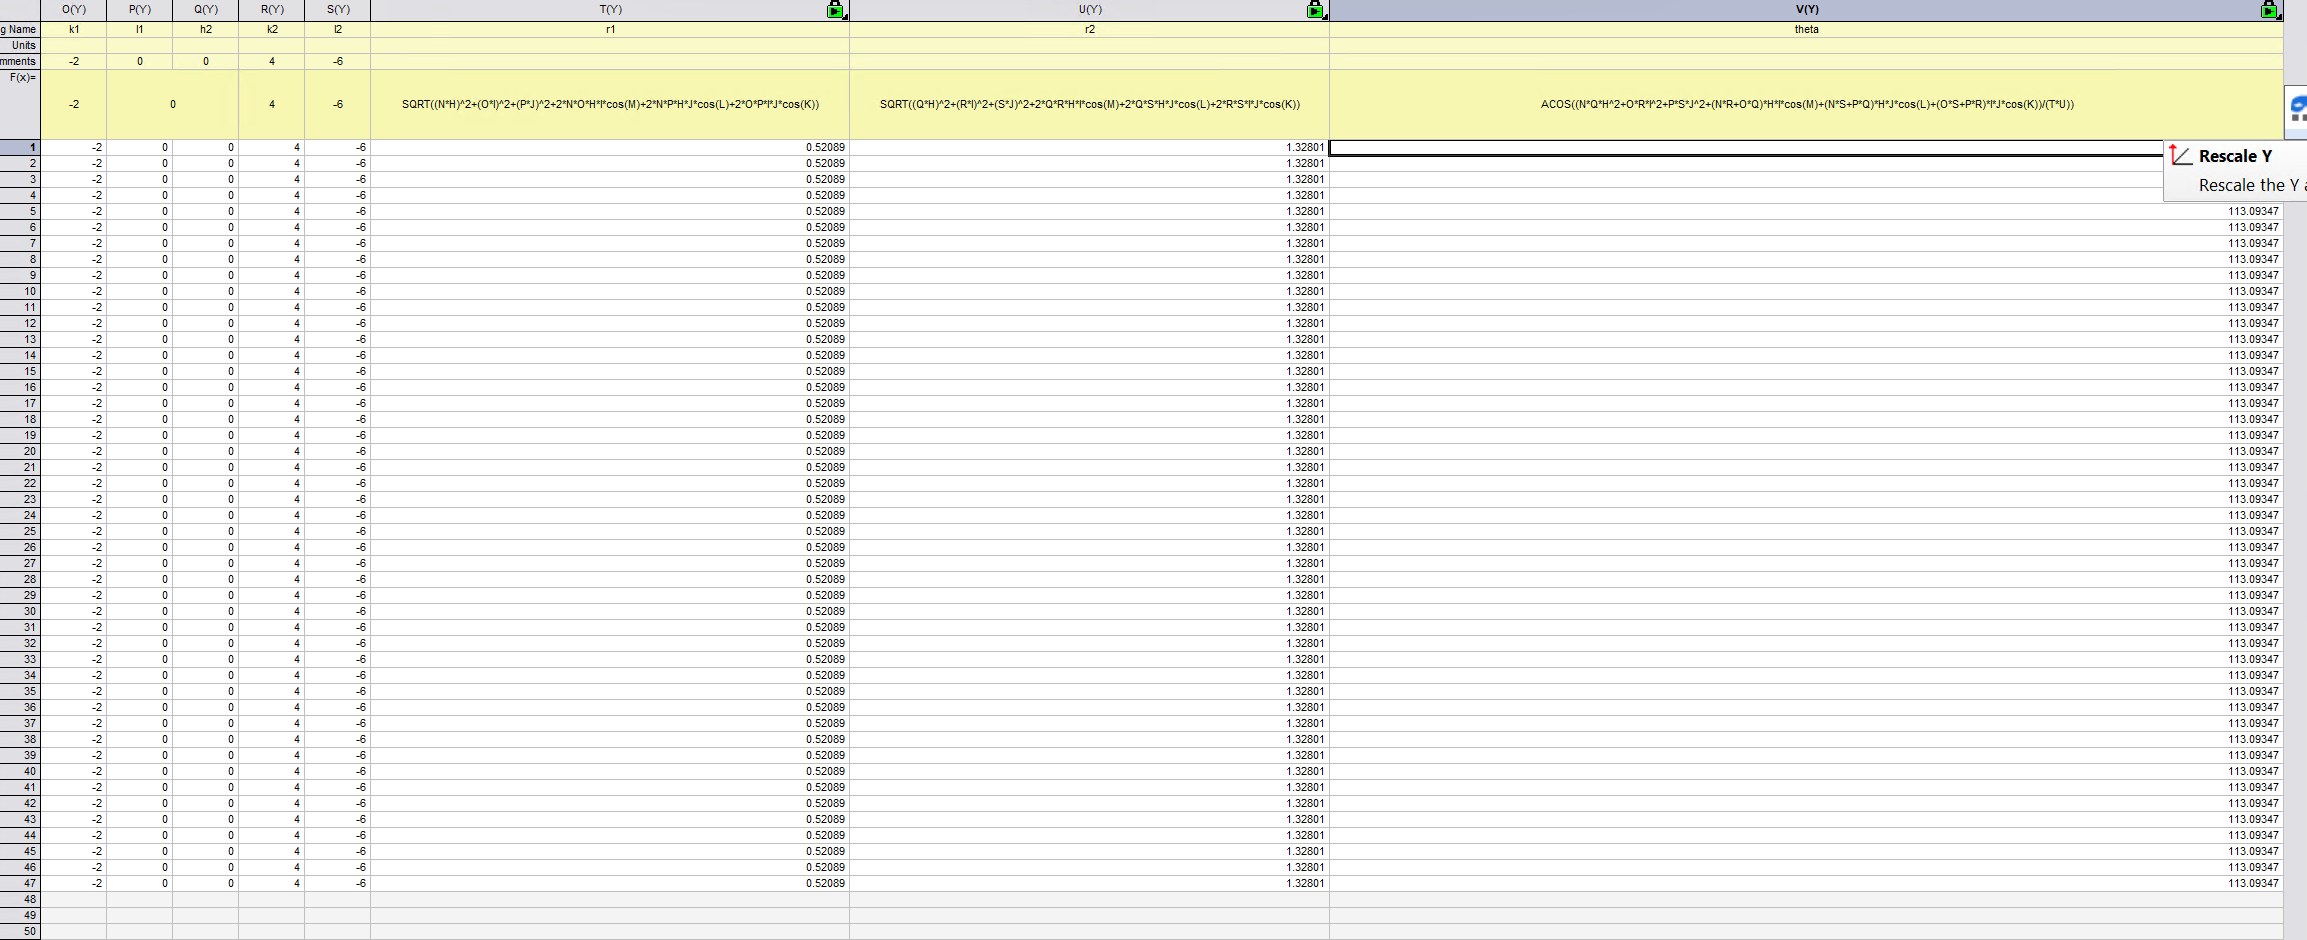
\includegraphics[width=\linewidth]{zone332/zone332_a.png}
    \caption{基矢与 $r_1,r_2,\theta$}
    \label{fig:zone332-a}
  \end{subfigure}\hfill
  \begin{subfigure}[t]{0.14\linewidth}
    \centering
    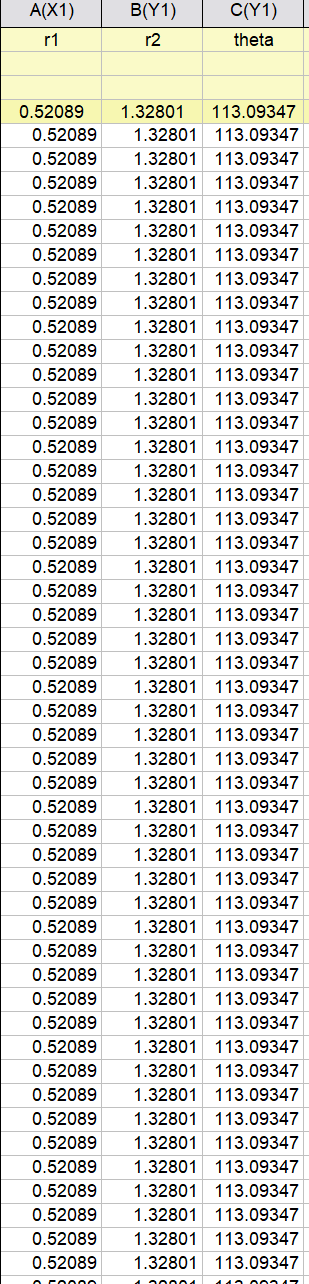
\includegraphics[height=4.3cm]{zone332/zone332_b.png}
    \caption{坐标复制}
    \label{fig:zone332-b}
  \end{subfigure}

  \vspace{0.3em}
  \begin{subfigure}[t]{0.48\linewidth}
    \centering
    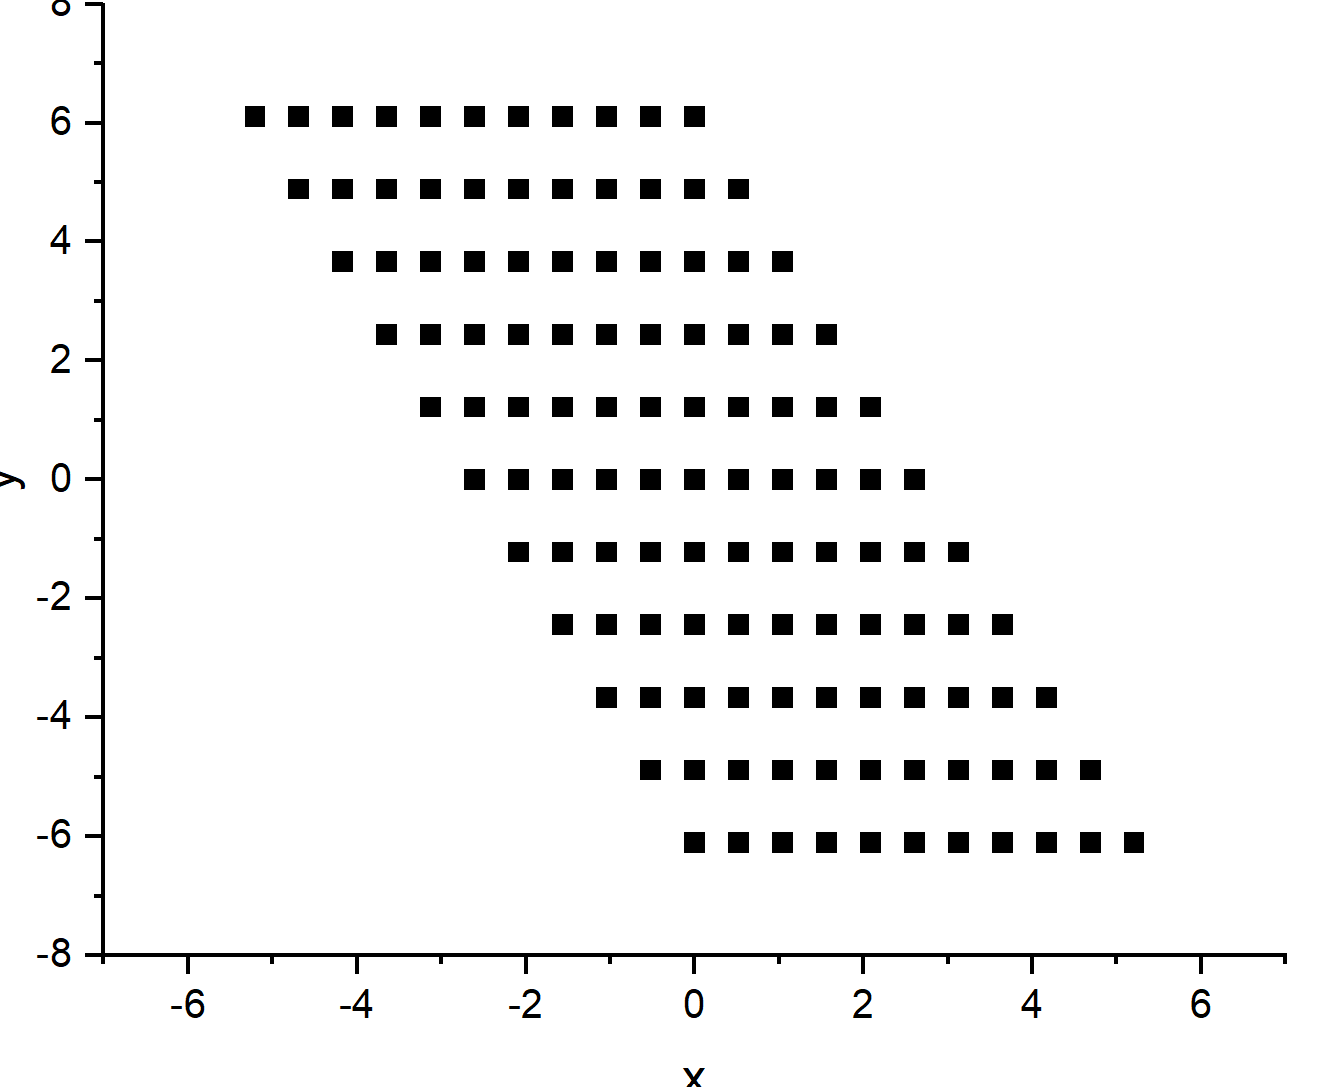
\includegraphics[width=\linewidth]{zone332/zone332_c.png}
    \caption{二维散点图}
    \label{fig:zone332-c}
  \end{subfigure}\hfill
  \begin{subfigure}[t]{0.48\linewidth}
    \centering
    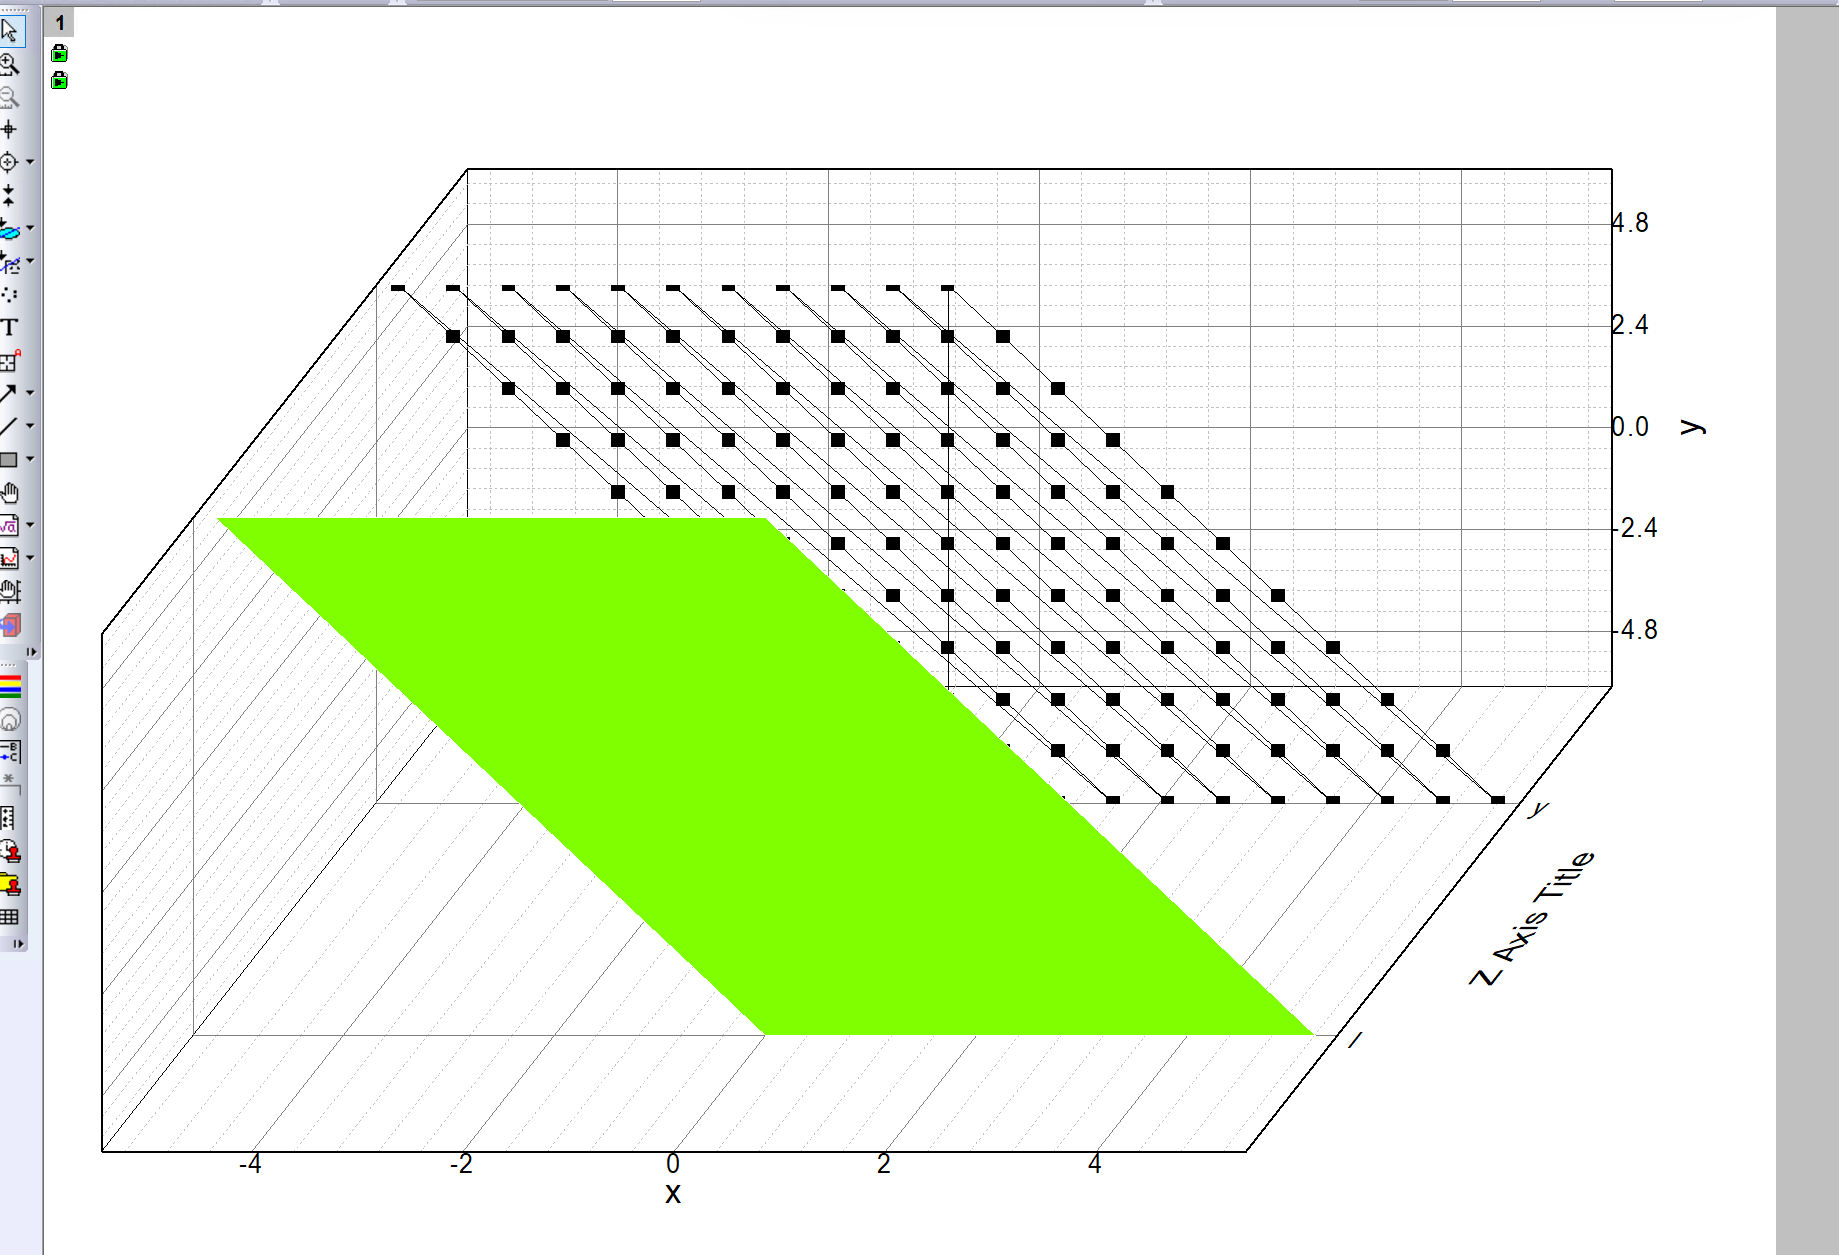
\includegraphics[width=\linewidth]{zone332/zone332_d.png}
    \caption{三维 Waterfall 图}
    \label{fig:zone332-d}
  \end{subfigure}
  \caption{[332] 带轴电子衍射模拟：(a) 基矢 $(2\bar{2}0)^*$、$(04\bar{6})^*$ 与 $r_1=0.52089$~\AA$^{-1}$、$r_2=1.32801$~\AA$^{-1}$、$\theta=113.0935^\circ$；(b) 坐标复制；(c) 斜方二维点阵；(d) 三维 Waterfall 图。}
  \label{fig:zone332}
\end{figure}

\subsubsection{[334] 带轴}

[334] 带轴的基矢为 $\bm{g}_1=(2\bar{2}0)^*$、$\bm{g}_2=(08\bar{6})^*$，$r_1=0.52089$~\AA$^{-1}$，$r_2=1.84162$~\AA$^{-1}$，$\theta=124.4499^\circ$。它与 [332] 共用 $\bm{g}_1=(2\bar{2}0)^*$，但 $\bm{g}_2$ 由 $(04\bar{6})^*$ 变为 $(08\bar{6})^*$，长度由 1.32801 增至 1.84162~\AA$^{-1}$，夹角由 $113.09^\circ$ 增至 $124.45^\circ$。因此 [334] 的点阵更“斜”，第二方向的点间距更大；允许的反射包括 220、331、440、531 等。

\begin{figure}[H]
  \centering
  \begin{subfigure}[t]{0.64\linewidth}
    \centering
    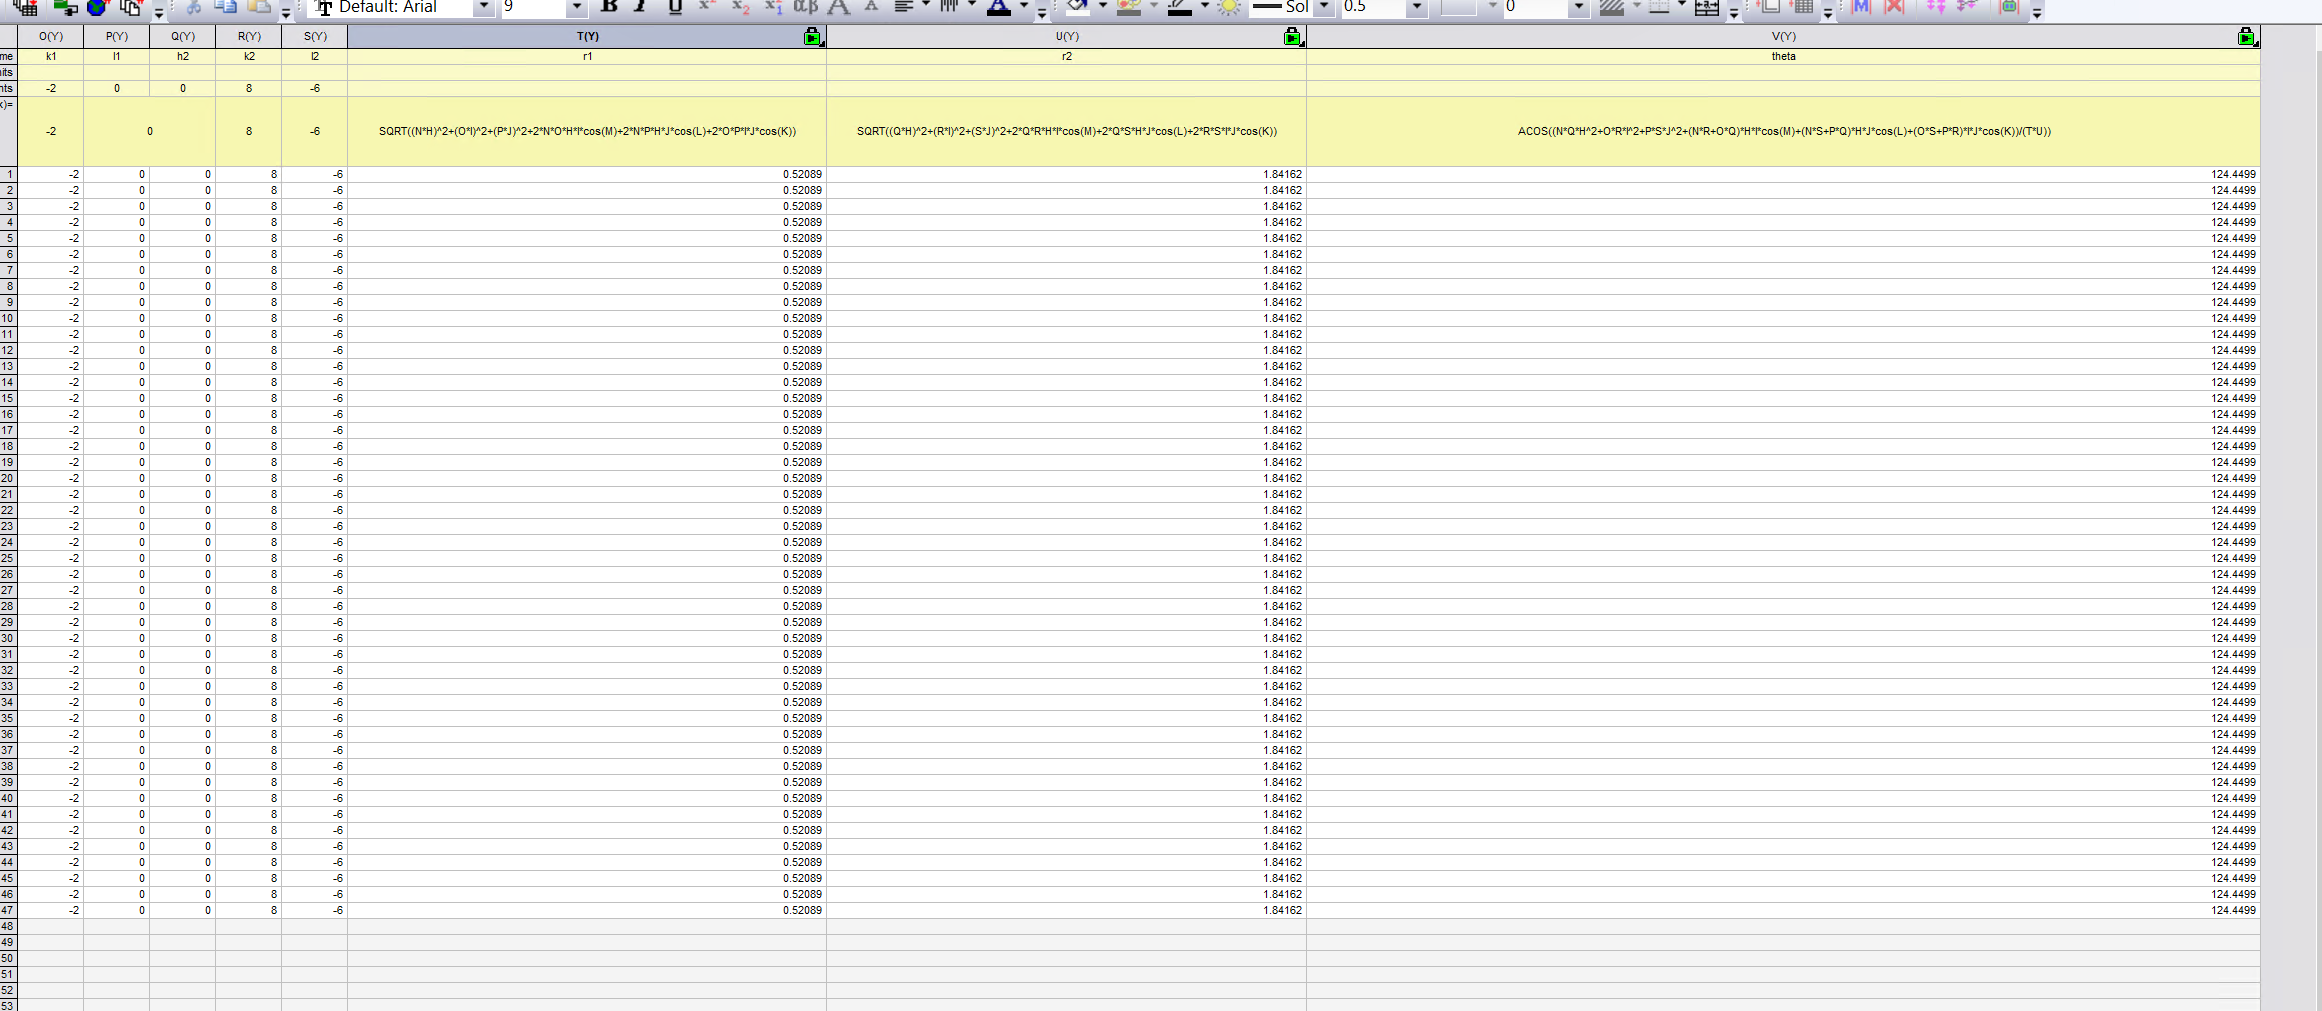
\includegraphics[width=\linewidth]{zone334/zone334_a.png}
    \caption{基矢与 $r_1,r_2,\theta$}
    \label{fig:zone334-a}
  \end{subfigure}\hfill
  \begin{subfigure}[t]{0.14\linewidth}
    \centering
    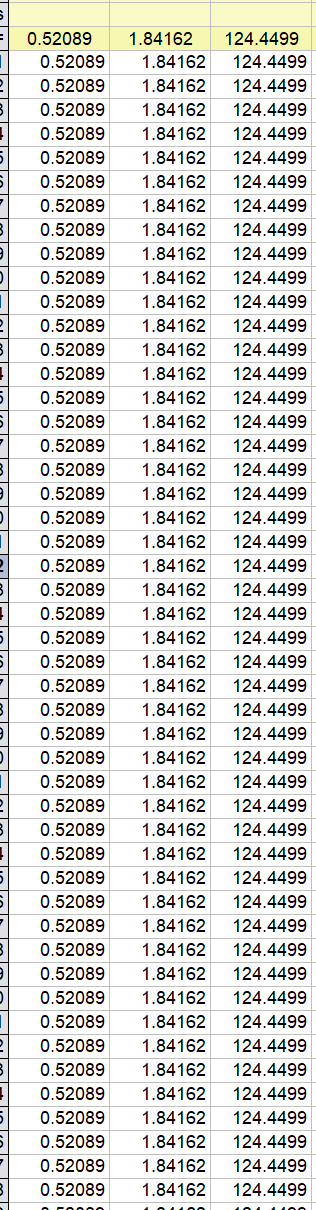
\includegraphics[height=4.3cm]{zone334/zone334_b.png}
    \caption{坐标复制}
    \label{fig:zone334-b}
  \end{subfigure}

  \vspace{0.3em}
  \begin{subfigure}[t]{0.48\linewidth}
    \centering
    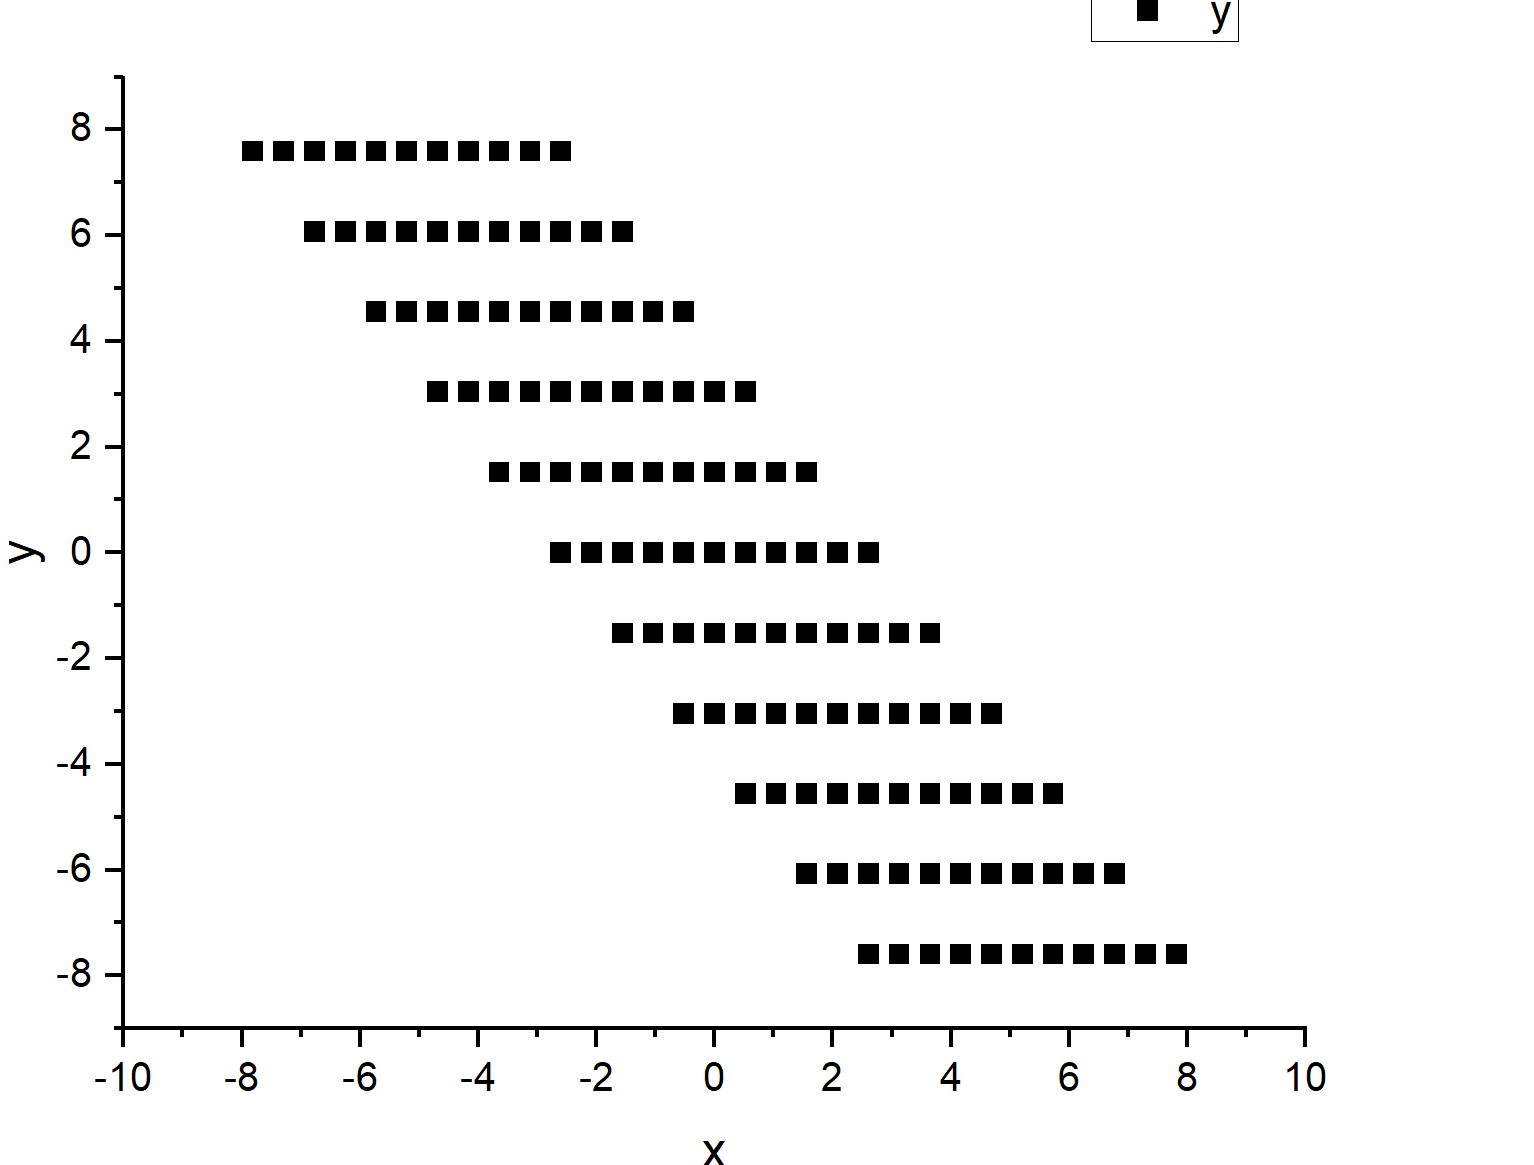
\includegraphics[width=\linewidth]{zone334/zone334_c.png}
    \caption{二维散点图}
    \label{fig:zone334-c}
  \end{subfigure}\hfill
  \begin{subfigure}[t]{0.48\linewidth}
    \centering
    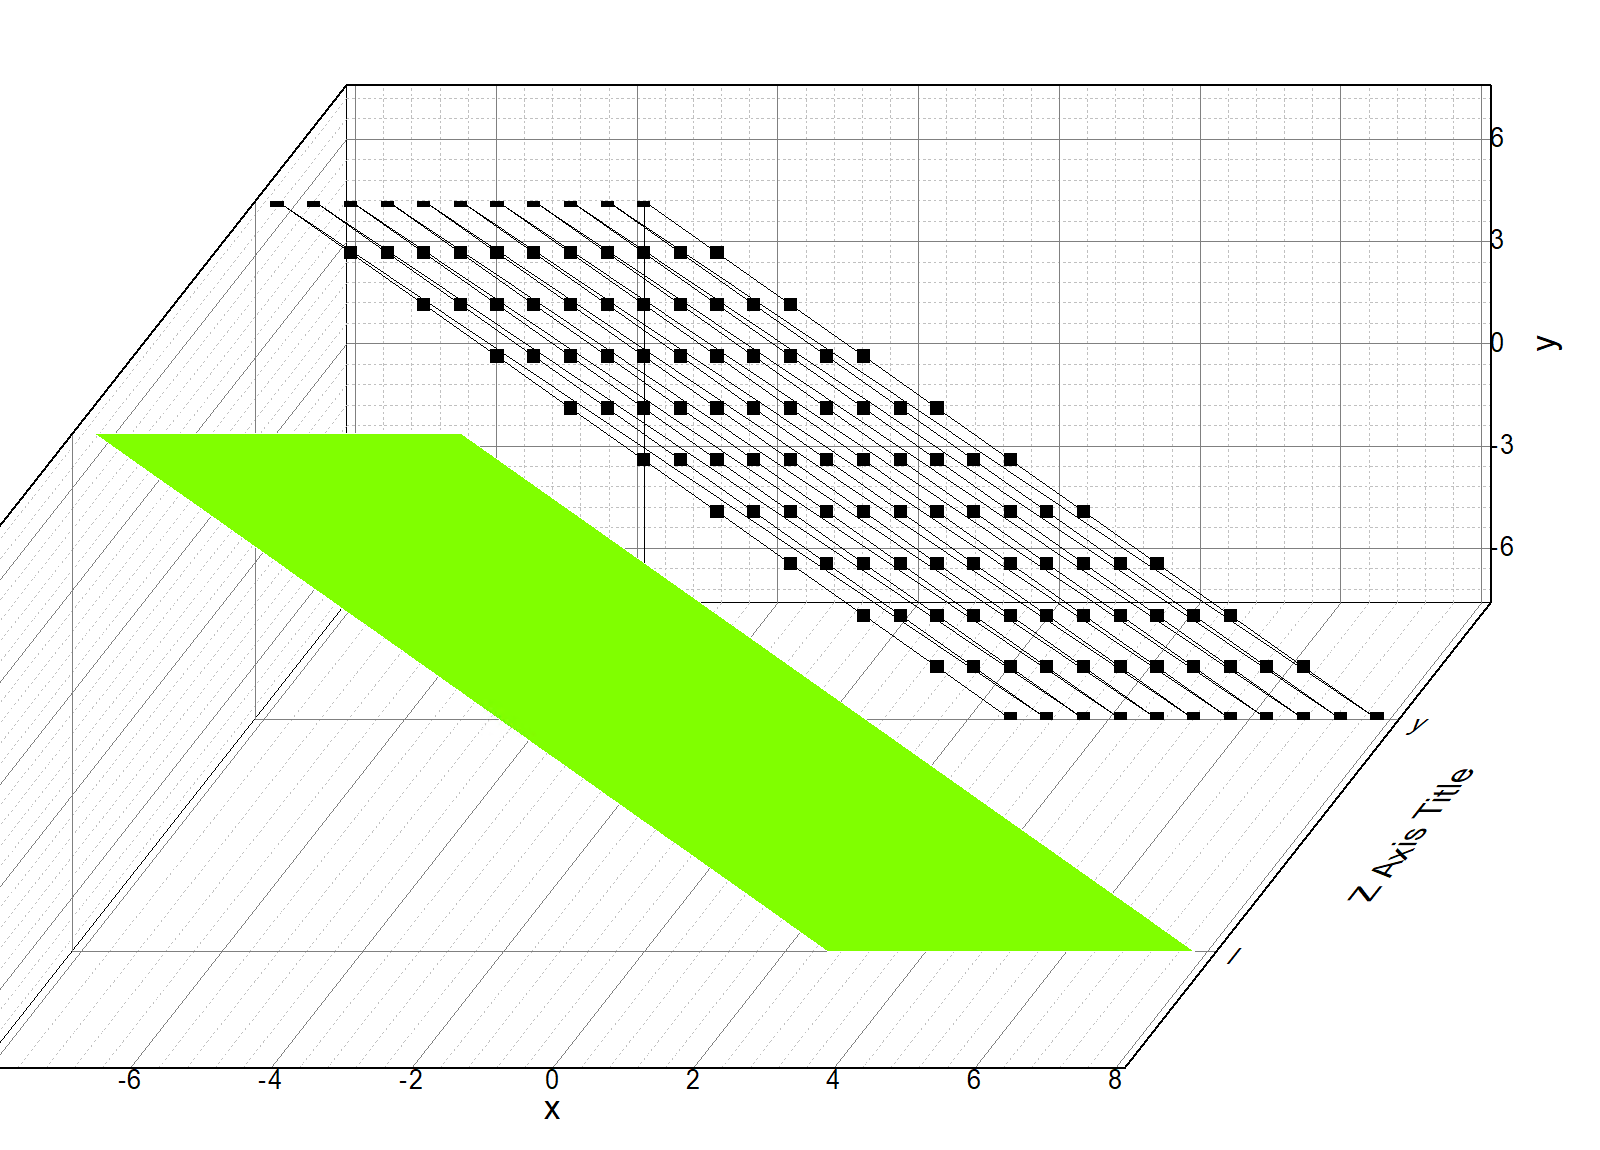
\includegraphics[width=\linewidth]{zone334/zone334_d.png}
    \caption{三维 Waterfall 图}
    \label{fig:zone334-d}
  \end{subfigure}
  \caption{[334] 带轴电子衍射模拟：(a) 基矢 $(2\bar{2}0)^*$、$(08\bar{6})^*$ 与 $r_1=0.52089$~\AA$^{-1}$、$r_2=1.84162$~\AA$^{-1}$、$\theta=124.4499^\circ$；(b) 坐标复制；(c) 斜方二维点阵；(d) 三维 Waterfall 图。}
  \label{fig:zone334}
\end{figure}

\subsubsection{[345] 带轴}

[345] 带轴的基矢为 $\bm{g}_1=(2\bar{4}2)^*$、$\bm{g}_2=(\bar{6}22)^*$，$r_1=0.90221$~\AA$^{-1}$，$r_2=1.22159$~\AA$^{-1}$，$\theta=119.4962^\circ$。这是五个带轴中指数最高、对称性最低的一个；$r_1$ 明显大于 [001] 和 [111]，因此视场内点数较少、点间距较大。允许的反射包括 311、331、422、531 等。图 \ref{fig:zone345}(c) 的二维点阵呈明显的斜方排列，图 \ref{fig:zone345}(d) 的三维 Waterfall 图也反映了同样的几何。

\begin{figure}[H]
  \centering
  \begin{subfigure}[t]{0.64\linewidth}
    \centering
    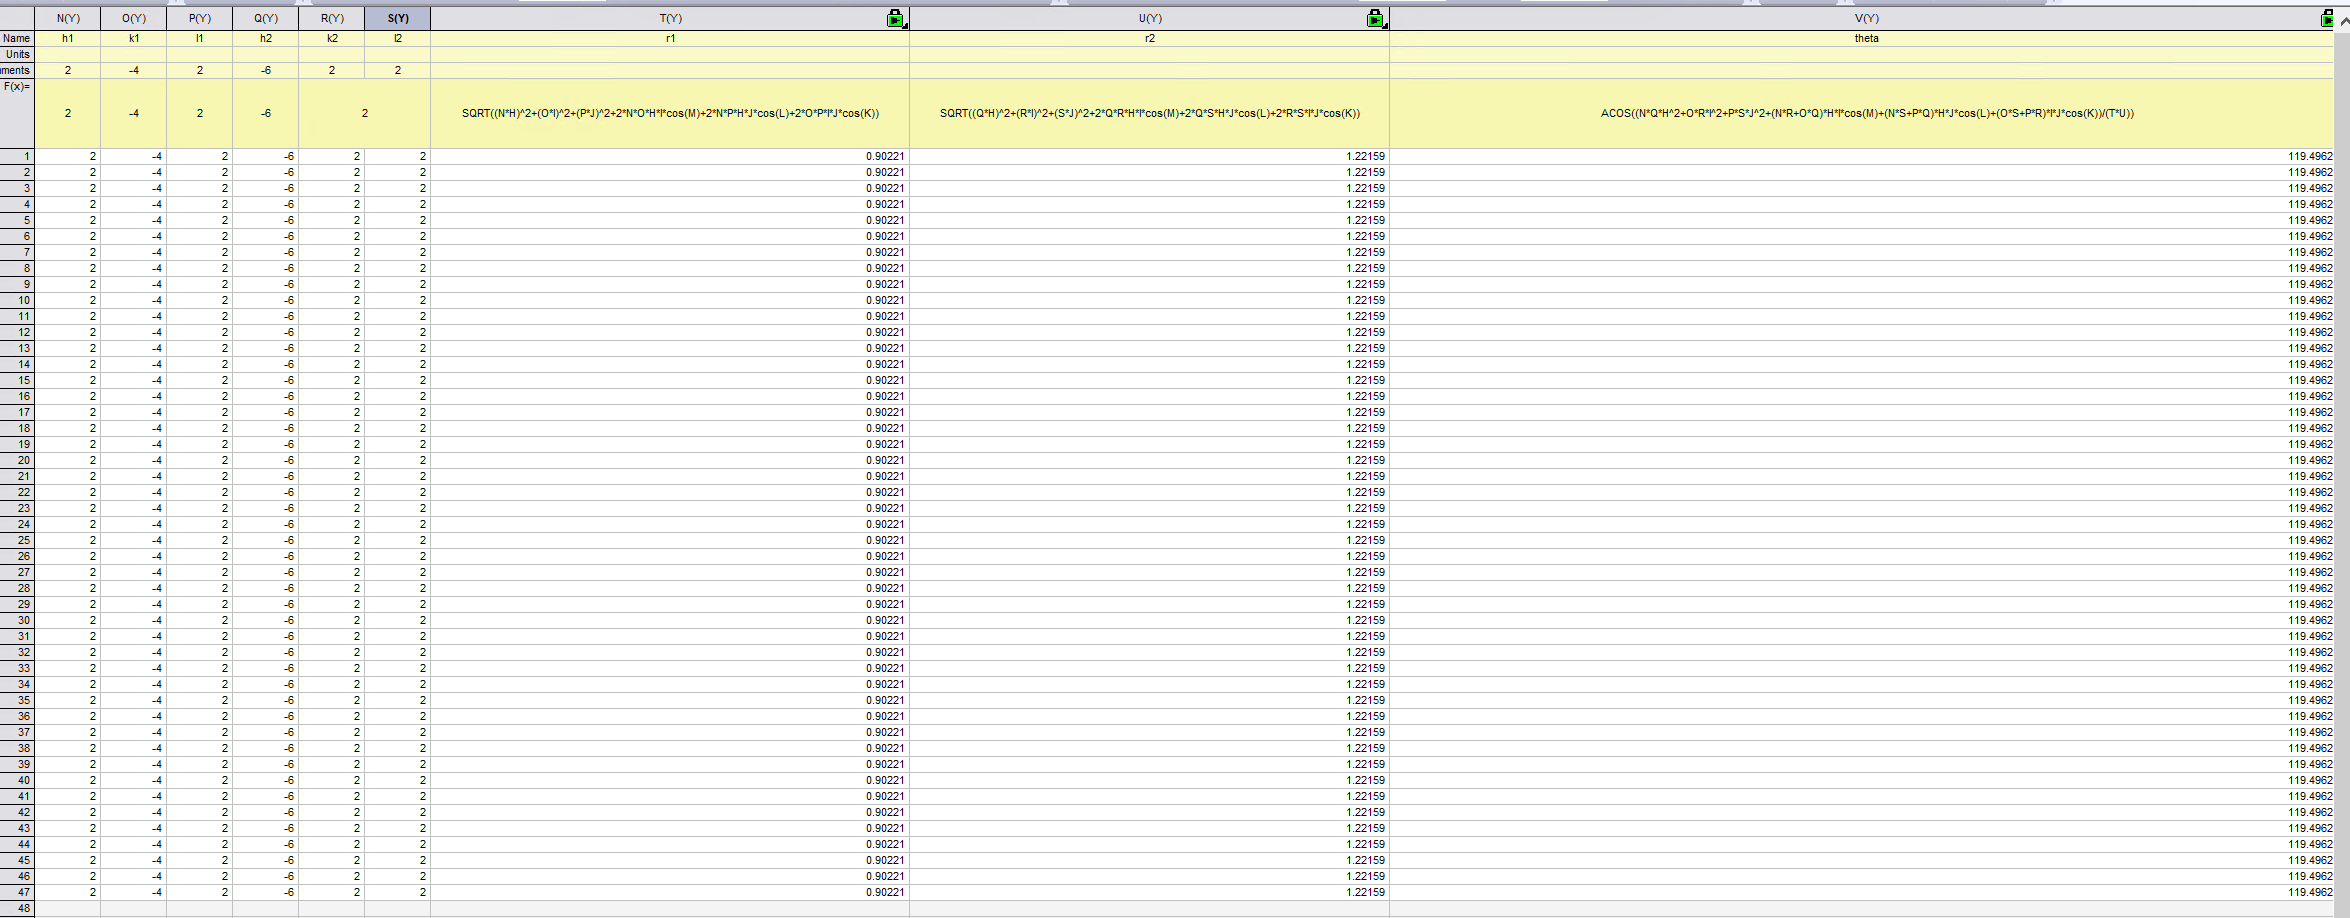
\includegraphics[width=\linewidth]{zone345/zone345_a.png}
    \caption{基矢与 $r_1,r_2,\theta$}
    \label{fig:zone345-a}
  \end{subfigure}\hfill
  \begin{subfigure}[t]{0.14\linewidth}
    \centering
    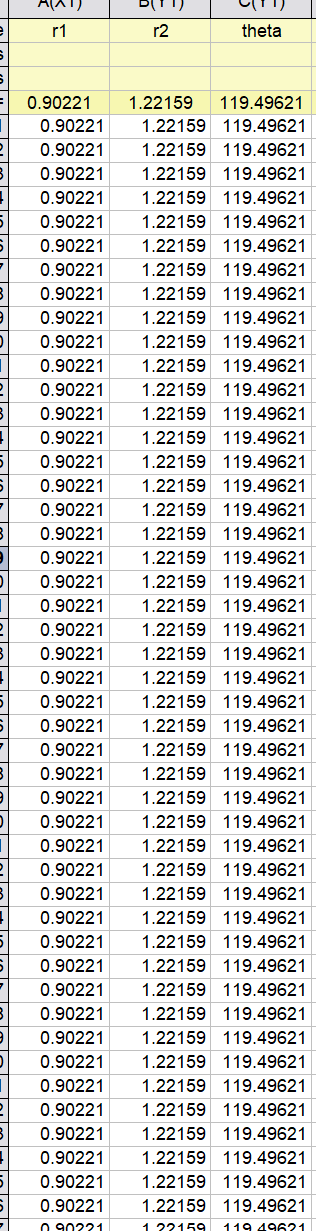
\includegraphics[height=4.3cm]{zone345/zone345_b.png}
    \caption{坐标复制}
    \label{fig:zone345-b}
  \end{subfigure}

  \vspace{0.3em}
  \begin{subfigure}[t]{0.48\linewidth}
    \centering
    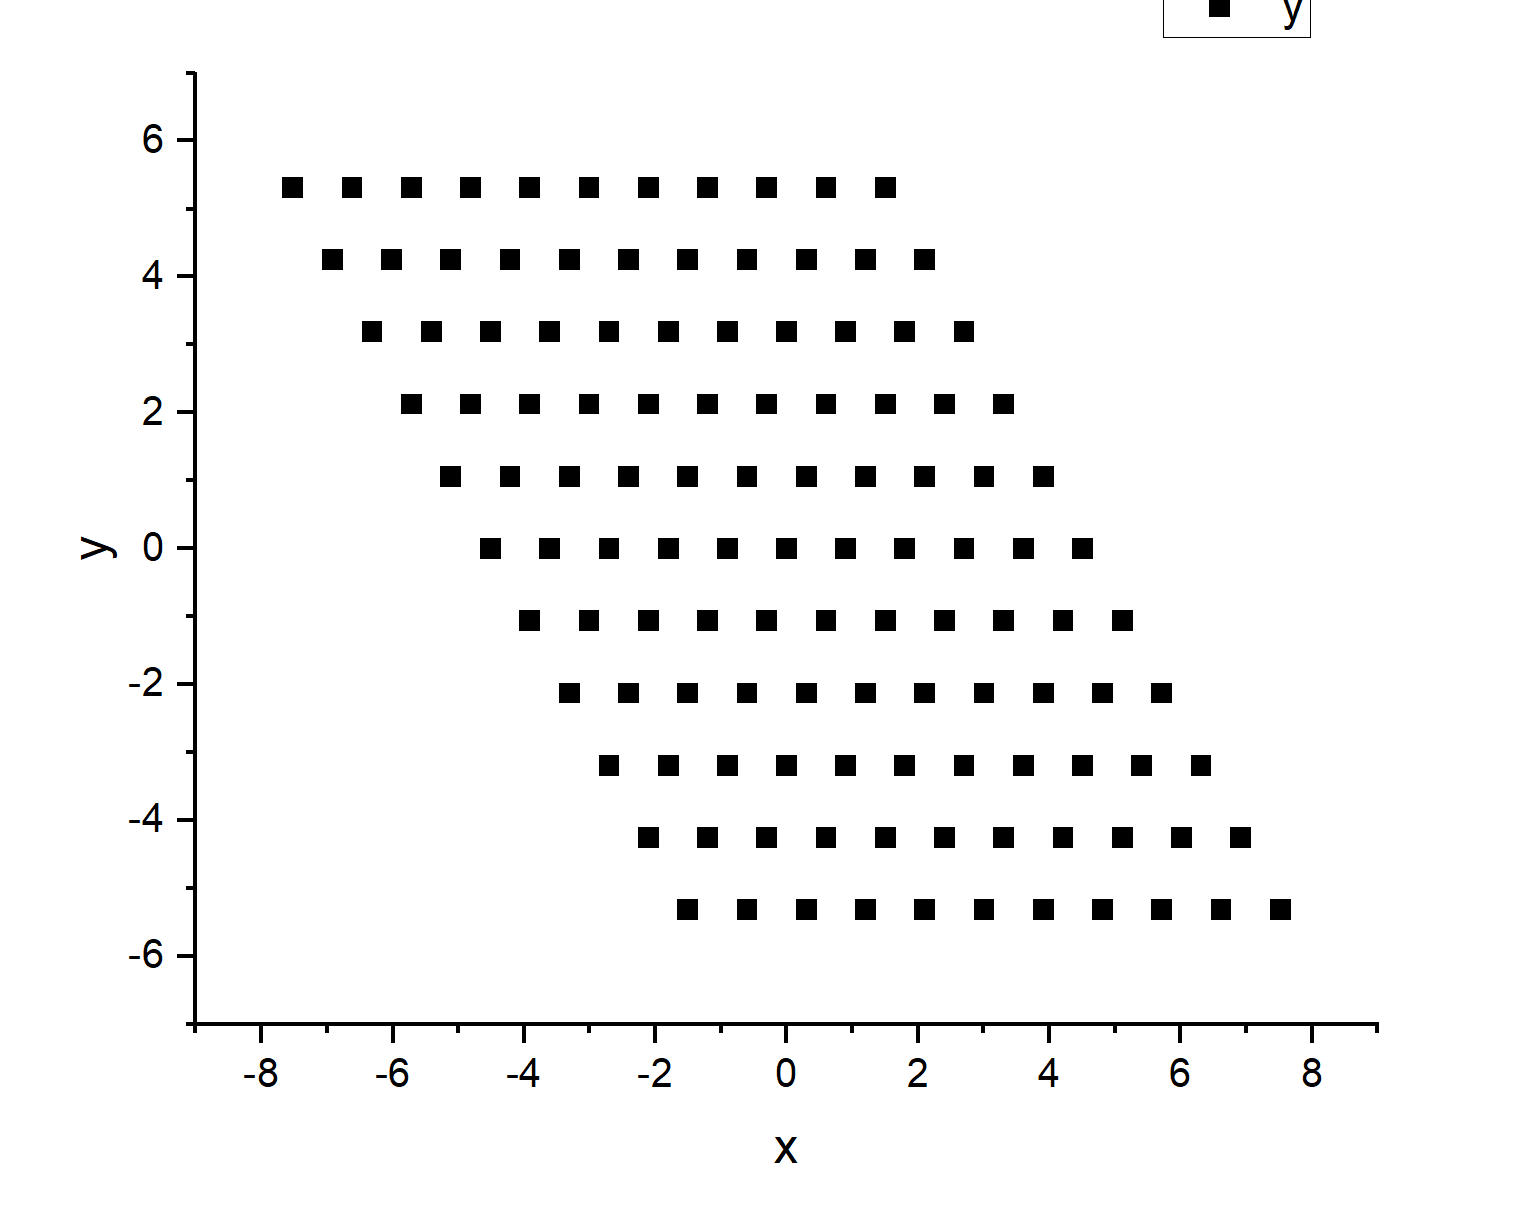
\includegraphics[width=\linewidth]{zone345/zone345_c.png}
    \caption{二维散点图}
    \label{fig:zone345-c}
  \end{subfigure}\hfill
  \begin{subfigure}[t]{0.48\linewidth}
    \centering
    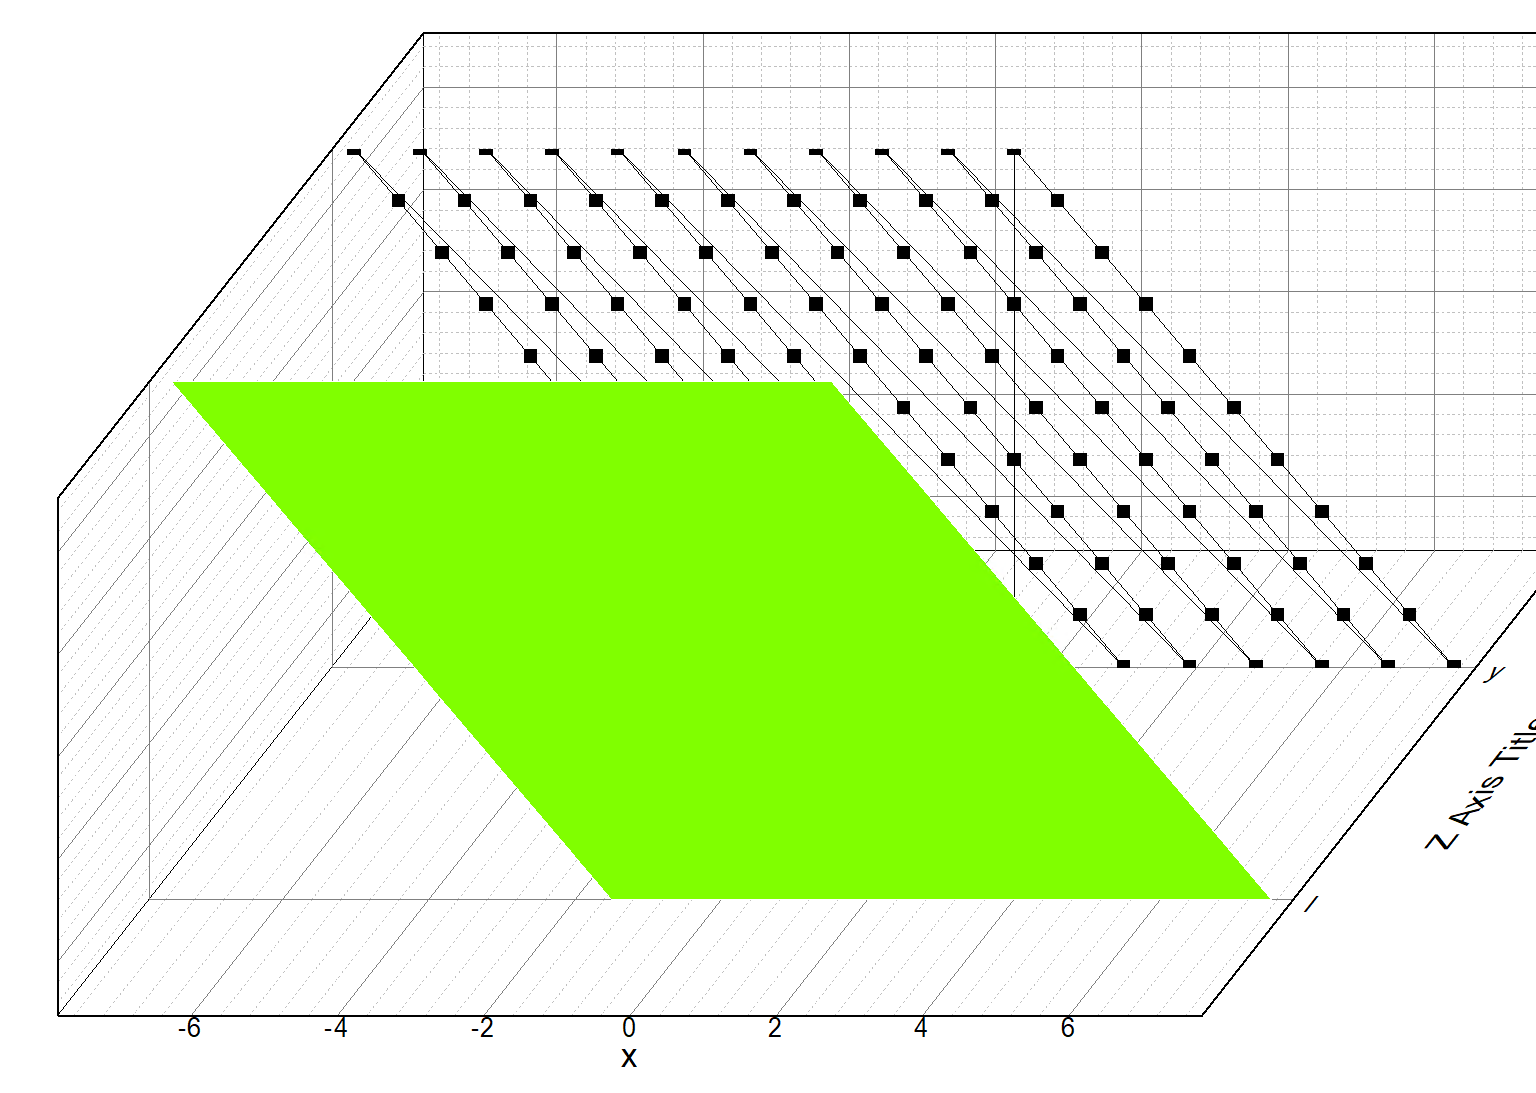
\includegraphics[width=\linewidth]{zone345/zone345_d.png}
    \caption{三维 Waterfall 图}
    \label{fig:zone345-d}
  \end{subfigure}
  \caption{[345] 带轴电子衍射模拟：(a) 基矢 $(2\bar{4}2)^*$、$(\bar{6}22)^*$ 与 $r_1=0.90221$~\AA$^{-1}$、$r_2=1.22159$~\AA$^{-1}$、$\theta=119.4962^\circ$；(b) 坐标复制；(c) 斜方二维点阵；(d) 三维 Waterfall 图。}
  \label{fig:zone345}
\end{figure}

\subsection{讨论}

把五个带轴放在一起比较，可以看到一条清晰的规律：带轴指数越低、对称性越高，二维点阵越规整；带轴指数越高，点阵越“斜”，点间距和夹角越不规整。表 \ref{tab:zone-summary} 汇总了五个带轴的几何参数、点阵类型和代表反射。[001] 是正方形点阵，[111] 是三角/六方点阵，这两个低指数带轴具有最高的对称性；[332] 和 [334] 共用 $\bm{g}_1=(2\bar{2}0)^*$，但第二条基矢不同，因此一个方向的点间距相同、另一个方向的点间距和夹角不同；[345] 的两条基矢都较长，视场内点数最少，斜方特征最明显。

从衍射强度的角度看，几何点阵只给出“可能出现”的位置，真正“出现”的斑点还要满足结构因子不为零。第 3 章的 110 消光计算（图 \ref{fig:extinction}）就是一个典型例子：它在几何点阵中有确定的位置，但 $h,k,l$ 奇偶混合使 $F=0$，强度在数值上为零。对单晶硅，实际允许的反射是 111、220、311、400、331、422、511/333、440 等；在 [001] 带轴中，100、110、200 等消光，220、400 等出现；在 [111] 带轴中，111 属于高阶劳厄带，零阶劳厄区内的强点是 220、422、440 等。

本模拟还有几点局限。第一，采用运动学近似，忽略了电子衍射的动力学效应（多次散射、厚度消光等），因此强点的相对强度只能作半定量参考。第二，结构因子计算取 $f=14$ 的常数原子散射因子，没有考虑 $f(s)$ 随角度的衰减和温度因子；若需要更接近实验的强度，可按式 \eqref{eq:cromer-mann} 把 $f$ 换成 $f(s)$，并加入 Debye--Waller 因子。第三，所选基矢不一定是最短的二维基矢，例如 [332] 的 $\bm{g}_2=(04\bar{6})^*$ 是 $(02\bar{3})^*$ 的两倍；若取最短基矢或允许 $m,n$ 取半整数，可以得到更完整的倒易点阵。第四，模拟中没有相机长度、比例尺和 HOLZ 线，实际 SAED 花样的标定还需要相机常数和仪器参数。尽管有这些简化，五个带轴的模拟结果已经能够正确反映点阵几何、对称性和消光规律，达到了预期的模拟效果。

\begin{table}[H]
  \centering
  \caption{五个带轴的点阵特征与代表反射汇总}
  \label{tab:zone-summary}
  \small
  \setlength{\tabcolsep}{4pt}
  \renewcommand{\arraystretch}{1.08}
  \begin{tabular}{cccccl}
    \toprule
    带轴 & $r_1$/\AA$^{-1}$ & $r_2$/\AA$^{-1}$ & $\theta$/$^\circ$ & 点阵 & 代表允许反射 \\
    \midrule
    {}[001] & 0.18416 & 0.18416 & 90.0000  & 正方 & 220, 400, 440, 620 \\
    {}[111] & 0.26044 & 0.26044 & 120.0000 & 三角/六方 & 220, 422, 440 \\
    {}[332] & 0.52089 & 1.32801 & 113.0935 & 斜方 & 220, 311, 331, 440 \\
    {}[334] & 0.52089 & 1.84162 & 124.4499 & 斜方 & 220, 331, 440, 531 \\
    {}[345] & 0.90221 & 1.22159 & 119.4962 & 斜方 & 311, 331, 422, 531 \\
    \bottomrule
  \end{tabular}
\end{table}
